%% Thesis template
%% PMC, University of Minho
%% if required, comment unused packages
\documentclass[12pt,english,oneside]{book}
% \usepackage[portuguese]{babel}
% \usepackage[utf8]{inputenc} 
\usepackage{times}
\usepackage[T1]{fontenc}
\usepackage[latin1]{inputenc}
\usepackage{a4wide}
\usepackage{fancyhdr}
\pagestyle{fancy}
\usepackage{subfigure}
\usepackage{float}
\usepackage{graphicx}
\usepackage{setspace}
\usepackage{algpseudocode, algorithm}
\usepackage{varwidth}
\usepackage{caption}
\usepackage{hyperref}
\usepackage{listings}
\usepackage{color}
\usepackage{cite}\onehalfspacing


\definecolor{dkgreen}{rgb}{0,0.6,0}
\definecolor{gray}{rgb}{0.5,0.5,0.5}
\definecolor{mauve}{rgb}{0.58,0,0.82}

\lstset{frame=tb,
  language=Python,
  aboveskip=3mm,
  belowskip=3mm,
  showstringspaces=false,
  columns=flexible,
  basicstyle={\small\ttfamily},
  numbers=none,
  numberstyle=\tiny\color{gray},
  keywordstyle=\color{blue},
  commentstyle=\color{dkgreen},
  stringstyle=\color{mauve},
  breaklines=true,
  breakatwhitespace=true
  tabsize=2
}

\hypersetup{
  citebordercolor=1 1 1,
  filebordercolor=1 1 1,
  linkbordercolor=1 1 1
}

\makeatletter

%%%%%%%%%%%%%%%%%%%%%%%%%%%%%% LyX specific LaTeX commands.
%% Bold symbol macro for standard LaTeX users
\newcommand{\boldsymbol}[1]{\mbox{\boldmath $#1$}}

\floatstyle{ruled}
\newfloat{algorithm}{tbp}{loa}
\floatname{algorithm}{Algorithm}

%%%%%%%%%%%%%%%%%%%%%%%%%%%%%% Textclass specific LaTeX commands.
 \usepackage{verbatim}
 \newenvironment{lyxlist}[1]
   {\begin{list}{}
     {\settowidth{\labelwidth}{#1}
      \setlength{\leftmargin}{\labelwidth}
      \addtolength{\leftmargin}{\labelsep}
      \renewcommand{\makelabel}[1]{##1\hfil}}}
   {\end{list}}

%%%%%%%%%%%%%%%%%%%%%%%%%%%%%% User specified LaTeX commands.
\usepackage{color}
\usepackage{colortbl}
\usepackage{url}
\input{epsf}
\newcommand{\single}{\renewcommand\baselinestretch{1.0}}
\newcommand{\onehalf}{\renewcommand\baselinestretch{1.5}}
\newcommand{\double}{\renewcommand\baselinestretch{2.0}}
\fancyhead{}
\fancyhead[LE]{\slshape \leftmark}
\fancyhead[RO]{\slshape \rightmark}
\cfoot{\thepage}
\setlength{\parskip}{2mm}

\usepackage{babel}
\makeatother
\begin{document}
\begin{minipage}[c]{1.0\columnwidth}%
\begin{doublespace}
\vspace{2cm}
\begin{center}{\huge A new Framework to enable rapid innovation in Cloud Datacenter through a SDN approach.}\end{center}{\huge \par}
\end{doublespace}

\vspace{2cm}
\begin{center}{\large Jos\'{e} Teixeira}\end{center}{\large \par}
\vspace{2cm}

\begin{quote}
\begin{center}A thesis submitted to the University of Minho in the
subject of Informatics, for the degree of
% or Doctor of Philosophy 
Master of Science, under scientific supervision of Prof. Stefano Giordano and Prof. Alexandre Santos\end{center}\vspace{3cm}

\end{quote}
\begin{singlespace}
\begin{center}University of Minho\end{center}

\begin{center}School of Engineering\end{center}

\begin{center}Department of Informatics\end{center}
\end{singlespace}

\begin{center}{\large September, 2013}\end{center}\end{minipage}%
\thispagestyle{empty}

\pagenumbering{roman}


\newpage


\chapter*{Acknowledgments}

\addcontentsline{toc}{chapter}{Acknowledgments}

% \noindent I would like...

% \medskip{}
% \noindent I also...

\chapter*{Abstract}

\addcontentsline{toc}{chapter}{Abstract}

\begin{singlespace}
\hspace{0.6cm}
In the last years, the widespread of Cloud computing as the main paradigm to deliver a large plethora of virtualized services significantly increased the complexity of Datacenters management and raised new performance issues for the intra-Datacenter network.
Providing heterogeneous services and satisfying users' experience is really challenging for Cloud service providers, since system (IT resources) and network administration functions are definitely separated.

As the Software Defined Networking (SDN) approach seems to be a promising way to address innovation in Datacenters, the thesis presents a new framework that allows to develop and test new OpenFlow--based controllers for Cloud Datacenters.
More specifically, the framework enhances both Mininet (a well--known SDN emulator) and POX (a Openflow controller written in python), with all the extensions necessary to experiment novel control and management strategies of IT and network resources.

Further more, the framework was validated by implementing and testing well known policies.
Hybrid allocation policies (considering both network and servers) were also implemented and scalability tests were performed.

\end{singlespace}

\paragraph{Keywords:}
Datacenter, Cloud, SDN, OpenFlow.

\newpage

\addcontentsline{toc}{chapter}{Contents}\tableofcontents{}

\clearpage

\chapter*{List of Acronyms}

\addcontentsline{toc}{chapter}{List of Acronyms}

\markboth{LIST OF ACRONYMS}{LIST OF ACRONYMS}

\begin{lyxlist}{00.00.0000}
\begin{singlespace}
\item [CPU]Central Processing Unit
\item [DC]Datacenter
\item [DCN]Datacenter Networks
\item [IO]Input\/Output
\item [IP]Internet Protocol 
\item [IT]Information Technology
\item [OF]Openflow
\item [OS]Operative System
\item [QoS] Quality of Service
\item [QoE] Quality of Experience
\item [RAM]Random-access Memory
\item [SDN]Software Defined Networking
\item [VM]Virtual Machine
\item [VMM]Virtual Machine Manager
\item [WAN] Wide Area Network
\end{singlespace}
\end{lyxlist}


\addcontentsline{toc}{chapter}{List of Figures}\listoffigures


\addcontentsline{toc}{chapter}{List of Tables}\listoftables


\setcounter{page}{0}

\pagenumbering{arabic}


\chapter{Introduction\label{cha:introduction}}

\section{Introduction}
\hspace{0.6cm}

A Cloud DC consists of virtualized resources that are dynamically allocated, in a seamless and automatic way, to a plethora of heterogeneous applications.
In Cloud DCs, services are no more tightly bounded to physical servers, as occurred in traditional DCs, but are provided by Virtual Machines that can migrate from a physical server to another increasing both scalability and reliability.
Software virtualization technologies allow a better usage of DC resources; DC management, however, becomes much more difficult, due to the strict separation between systems (\textit{i.e.}, server, VMs and virtual switches) and network (\textit{i.e.}, physical switches) administration.

Moreover, new issues arise, such as isolation and connectivity of VMs.
Services performance may suffer from the fragmentation of resources as well as the rigidity and the constraints imposed by the intra-DC network architecture (usually a multilayer 2-tier or 3-tier fat-tree composed of Edge, Aggregation and Core switches\cite{dc_arch}).
Therefore, Cloud service providers (\textit{e.g.},\cite{amazon}) ask for a next generation of intra-DC networks meeting the following features: 1) efficiency, \textit{i.e.}, high server utilization; 2) agility, \textit{i.e.}, fast network response to server/VMs provisioning; 3) scalability, \textit{i.e.}, consolidation and migration of VMs based on applications' requirements; 4) simplicity, \textit{i.e.}, performing all those tasks easily\cite{baldonado}.

In this scenario, a recent approach to programmable networks (\textit{i.e.}, Software-Defined Networking) seems to be a promising way to satisfy DC network requirements\cite{ibmnec}. 
Unlike the classic approach where network devices forward traffic according to the adjacent devices, SDN is a new network paradigm that decouples routing decisions (control plane) from the traffic forwarding (data plane). This routing decisions are made by a programmable centralized intelligence called controller that helps make this architecture more dynamic, automated and manageable.

Following the SDN--based architecture the most deployed SDN protocol is OpenFlow\cite{openflow}\cite{onf}, and it is the open standard protocol to communicate and control OF-compliant network devices.
Openflow allows a controller to install into OF--compliant network devices forwarding rules which are defined by the administrator/network engineer and match specific traffic flows.

Since SDN allows to re-define and re-configure network functionalities, the basic idea is to introduce an SDN-cloud-DC controller that enables a more efficient, agile, scalable and simple use of both VMs and network resources.
Nevertheless, before deploying the novel architectural solutions, huge test campaigns must be performed in experimental environments reproducing a real DC.
To this aim, a novel framework is introduced that allows to develop and assess novel SDN-Cloud-DC controllers, and to compare the performance of control and management strategies jointly considering both IT and network resources\cite{im2013}.

% \begin{quote}''OpenFlow allows, for the first time, an external control plane to abstract the entire underlying network fabric so that fabric is universally addressable and all topology and state information is commonly managed''{ --- \textup{ Jason Matlof}, vice president of marketing at Big Switch}\end{quote}

% \newpage
\section{Motivation and objectives\label{sec:motobj}}
\hspace{0.6cm}

Although SDN came as a solution to fulfill the network requirements of the DCs, the only point of interaction with the IT resources is the generated traffic.
By definition SDN does not go further, but if there could be a controller that manages both IT and network resources, all the information could be shared easily and both of them could greatly benefit: the network could start to anticipate IT actions and adapt itself to have higher performance, more redundancy, etc; the IT because the resources could be better managed so that the network, not only stops being the bottleneck, but actually helps the IT complete the tasks faster and without affecting adjacent resources.

When developing an Openflow controller, the administrator/network engineer goals are to implement the desired behaviour and to test it (making sure it suits the requirements).
The currently available controllers already provide some abstraction, which varies according to the type of programming language, but they are still too low level to allow rapid innovation. 
Following the implementation, tests campaigns must be performed and for it a controlled environment should be set.
Although Openflow allows the use of slices of the real network for testing purposes, it is more convenient to use an emulator since the DC size can be dynamic, different scenarios can be easily produced and it only needs a single computer -- Mininet is such an emulator.
Despite its flexible API, Mininet does not provide any type of traffic generator and is not DC--oriented: poor topology generation regarding DCs; no support for VMs;

A whole framework composed by a modified OF controller that allows the access to both IT and network resources through an easy-to-use but full featured API, and a testing environment that communicates with it to provide a real DC emulation is the the main objective.
With this is is expected to endue the administrator/network engineer with all the tools needed to quickly develop, test and deploy VM and network management strategies into a DC.

% When the admin wants to try new DC VM allocation algorithms, first it takes to long to develop since the current controllers are still low level, and second if they want to test, or they try on their own DC (which could compromise the normal functioning and unless they try on a small part of the DC the result wont be accurate since they would be influences by the usual workload.
% Or they would use simulators(the problem with simulator is that usually you have to rewrite the algorithms that you will implement, and the results might not be accurate (correspond to the real environment)).
% At the same time, a whole framework that provides support to develop and test only the logic that the admin wants would also be cool, since they could focus on making new VM allocations that consider multiple factor (this is where OF helps since it has info about network)
% Maybe also talk a little about allowing to be easily expandable, extended.

% \begin{itemize}
% 	\item Understanding the basic features of SDN paradigm
% 	\item Studying the problematics in cloud DC VM allocations
% 	\item Apply the SDN paradigm to better exploit the DC resources
% 	\item Develop a framework for Cloud Datacenter emulation and new VM allocation policies
% 	\item ...
% \end{itemize}


\section{Thesis layout}
\hspace{0.6cm}

This thesis is structured into five chapters: the present Chapter \ref{cha:introduction} is a brief introduction of the proposed work, its motivation and objectives; the second is the state of art, it addresses the currently available solutions relating innovation in DCs, OF controllers and VM allocation and migration algorithms; the third one fully describes the framework, its evolution, extensions and how it can be used; in the forth chapter is presented the framework validation, the results of a hybrid allocation algorithm and performance tests; and in the last chapter are made conclusions about the developed work, as well as suggestions for future work.



\chapter{State of art \label{cha:stateofart} }

\section{Available solutions}

A number of research efforts have focused on novel solutions for emulation/simulation of Cloud DCs.
The available solutions provide a reference and material to analise and explore the concepts addressed along this thesis. 
This section presents and overview of them, highlighting their architecture, features and limitations.

\subsection{CloudSim}
\hspace{0.6cm}

Calheiros et al.\cite{cloudsim} proposed a Java-based platform, called Cloudsim, that allows to estimate cloud servers performance using a workflow model to simulate applications behaviour.
By providing a framework for managing most key aspect of a Cloud infrastructure (DC hardware and software, VM placement algorithm, Applications for VM, Storage access, Bandwidth provisioning) and by taking into consideration factors as energy-aware computational resources and costs, it helps to identify possible bottlenecks and improve overall efficiency.

Regarding the network aspect of Clousim, Garg et al.\cite{cloudsim2} extended such a system with both a new intra--DC network topology generator and a flow--based approach for collecting the value of network latency. However, in such a simulator, networks are considered only to introduce delay, therefore it is not possible to calculate other parameters (\textit{e.g.}, Jitter).
A SDN extension for Cloudsim as already been thought, Kumar et al.\cite{cloudsim3}, but it still just an architecture design, meaning it has not been implemented yet.

Although it allows to predict how the management strategies will behave, as a simulator, it does not allow to run real applications and deploying the tested management logic in a real environment still requires everything to be developed.

\subsection{FPGA Emulation}
\hspace{0.6cm}

Ellithorpe et al.\cite{box} proposed, a FPGA emulation platform that allows to emulate up-to 256 network nodes on a single chip.
\begin{quotation}
''Our basic approach to emulation involves constructing a model of the target architecture by composing simplified hardware models
of key datacenter building blocks, including switches, routers, links, and servers. Since models in our system are implemented in programmable hardware, designers have full control over emulated buffer sizes, line rates, topologies, and many other network properties.''

\hfill Ellithorpe et al.\cite{box}
\end{quotation}

This platform also allows the emulation of full SPARC v8 ISA compatible processor, which along with full system control provides a greater system visibility.
However, hardware programming skills might be a requirement and the cost of a single board is approximately 2, 000 dollars making this solution less attractive than ones based on just open--source software.

\subsection{Meridian}
\hspace{0.6cm}

Following the new shiny SDN paradigm, Banikazemi et al.\cite{meridian} proposed Meridian, an SDN--based controller
framework for cloud services in real environments.

\begin{figure}[htbp]
        \centering
        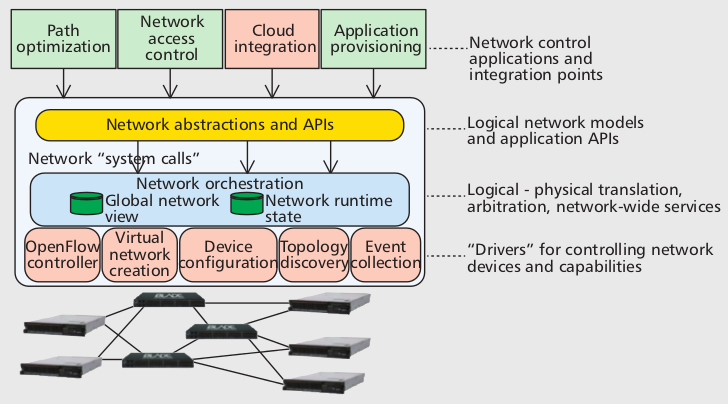
\includegraphics[width=0.8\textwidth]{figures/meridian_arch.png}
        \caption{Meridian SDN cloud networking platform architecture (Banikazemi et al.\cite{meridian})}
        \label{fig:meridian_arch}
\end{figure}

As shown in figure \ref{fig:meridian_arch}, the architecture is divided into three main layers: Network abstractions and API, where the network information can be accessed and manipulated (\textit{e.g.} access controlling policies, prioritizing traffic); Network Orchestration, translates the command provided by the API into physical network commands and orchestrates them for more complex operations. it also reveals the network topology and its variations; finally the ''drivers'' layer is an interface for underlying the network devices so several network devices and tools can be used.

Generally, this platform allows to create and manage different kind of logical network topologies and use their information for providing a greater control of the DC.
But as it works on top of a cloud Iaas platform (i.e., Openstack\cite{openstack}, IBM SmartCloud Provisioning\cite{scp}), it is limited to their management strategies and is only useful if one already has this type of infrastructure. Not having a testing environment is also a downside since the normal operation of the real DC can be compromised and also alter the testing results.

\subsection{ICanCloud, GreenCloud and GroudSim}
\hspace{0.6cm}

Other well--known open--source cloud simulators are ICancloud\cite{icancloud}, GreenCloud\cite{greencloud} and GroudSim\cite{groudsim}, but in none of them SDN features are available.

\newpage
\subsection{Mininet}
\hspace{0.6cm}
\begin{quotation}

''Mininet is a network emulator which creates a network of virtual hosts, switches, controllers, and links. Mininet hosts run standard Linux network software, and its switches support OpenFlow for highly flexible custom routing and Software-Defined Networking.''

\hfill Mininet \cite{mininet}
\end{quotation}

As a network emulator for SDN systems, mininet can generate OF compliant networks that connect to real controllers without the need of hardware resources. Such features derives from the use of Open vSwitch and enables the assessment of the operation of an OF controller before its deployment in a real environment.

It also provides tools for automatically generating topologies, however, as they can be basic, an API is available to reproduce any type of topology and experiments.
Mininet hosts behave just like real hosts, can run any program as long as it does not depend on non linux kernels, and can send packets through emulated interfaces.
But as they share the same host file system and PID space, a special attention is required when killing/running programs.

Despite its flexibility, Mininet lacks of a complete set of tools that easily allow to emulate the behaviour of a cloud DC, thus raising the following questions:
 
\begin{itemize}
\item How to easily generate and configure typical DC topologies?
\item How to simulate VMs allocation requests?
\item How to emulate the inter and in/out DC traffic?
\end{itemize}

\newpage
\section{Openflow Controllers}
\hspace{0.6cm}


\newpage
\section{Virtualization Platforms}
\hspace{0.6cm}
% Uncomment to include file.pdf
%\begin{figure}%[H]
%\begin{center}\includegraphics[scale=0.8]{file}\end{center}
%\caption{Legend \label{fig:LABEL}}
%\end{figure}


\chapter{The Framework \label{cha:framework} }

\section{Requirements}
\hspace{0.6cm}

Provide the user with a full package for the development and test of DC SDN Controller was one of the main purposes of the framework.
Aiming for such goal, but without discarding the deployment in a real DC, a single software platform was designed and developed.
Because the requirements change according to the controller being in the development or the deployment phase, so should the platform by creating and environment that best suits each of them.

\paragraph{Development \& Testing Phase}
\hspace{0.6cm}

Encourage a rapid development is one of the main requirements since it promotes innovation in the cloud DC.
It must be simple and fast to develop the desired logic, which can be achieved by providing easy access to information and management of the network and servers.
More specifically, automatic topology detection (and changes in it) associated with a high level API for accessing and managing switch's and server's information and statistics.

When testing, the framework should provide an automatic way of generating the VM requests and the traffic associated to each request (for testing the VM allocation and the network behaviour).
The traffic generator should also correctly represent the DC traffic profiles.
Allowing an easy access outside the controller for the statistics is also important, so it is possible to analyze the logic effects on the DC.

\paragraph{Deployment Phase}
\hspace{0.6cm}

For the deployment, the framework should be easy to configure and monitor, and no extra effort should be made for the framework to run on the real DC (it should adapt automatically). There should also be an intuitive way to make manual VM requests, so clients can generate and manage their own VMs.

\section{Chosen technologies}

\subsubsection{Openflow Controller: POX}
\hspace{0.6cm}

Being POX a python derivative of the NOX controller, which was developed by the same people who developed the Openflow protocol, adopting it would be a surplus since there is a higher chance it will continue to support Openflow, and that the new versions/features are available as soon as possible.
Besides, being a high level (comparing to C and C++), object and event oriented programming language, helps to create the abstraction level required for agile development and to make a more interactive controller.

\subsubsection{Datacenter Emulator: Mininet}
\hspace{0.6cm}

Mininet comes recommended in the Openflow tutorials as the platform for testing the OF compliant controllers.
It also provides an API in python for the development of custom made topologies and specific experiments, which along with the capacity that the virtualized hosts have of running almost any program, makes it a powerful platform.

\subsubsection{Virtualization platform: XCP 1.6 (Xen Cloud Platform)}
\hspace{0.6cm}

As a free and opensource platform though for the cloud, XCP bring all the features belonging to Xen, plus it comes with ready-to-install images, making it simpler to install and configure.
Having multiple interaction option is also an attractive feature, but having a Xen python API was decisive since hit gives the possibility to write all the code in one programming language which helps keeping the platform consistent.
\newpage

\section{Framework architecture}
\hspace{0.6cm}

\begin{figure}[htbp]
        \centering
        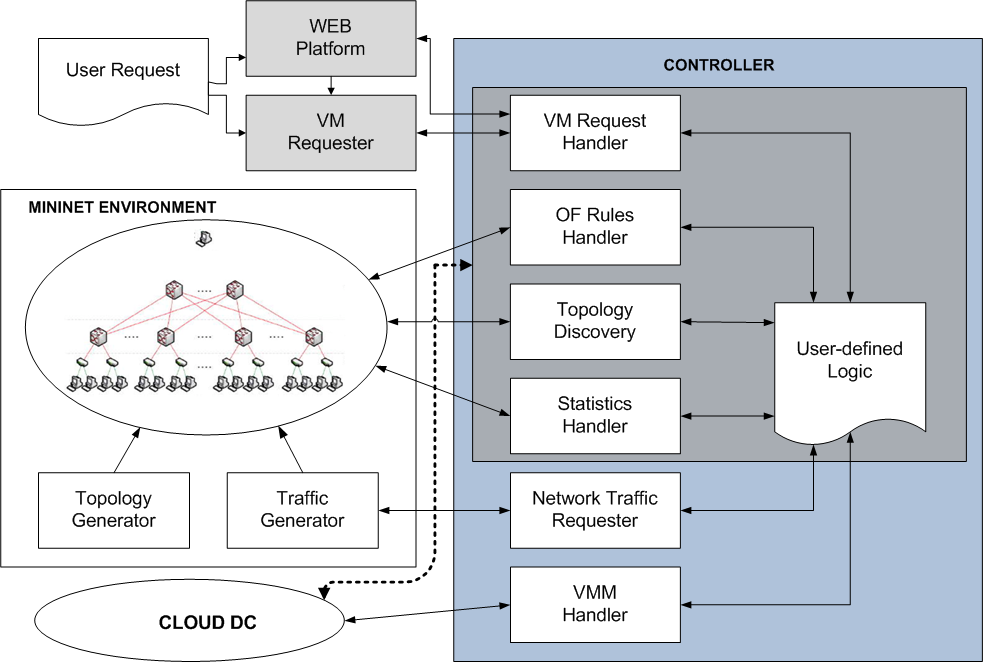
\includegraphics[width=0.8\textwidth]{figures/emulator_new.png}
        \caption{Framework Architecture}
        \label{fig:framework}
\end{figure}

The framework architecture, shown in figure \ref{fig:framework}, gives an overview of the its modules and their interaction.
The framework is divided into two main parts: the mininet environment - an extended version of mininet; and the controller - a modified, improved version of POX;

The mininet environment is made to be only used when testing the controller.
It is composed by the mininet platform with two extra modules that explore its API.
One of them is the {\it Topology Generator}, which allows to easily create multilayer 2-tier or 3-tier fat-tree DC topologies.
The other one is the {\it Traffic Generator} that allows to correctly simulate the allocation of VM into each server by generating traffic from that server to the exterior of the DC. It also allows to simulate inter VM communication.

As for the controller, it automatically manages the modules in order to only use the ones that are needed for each phase (development and testing or deployment).
Depending on it, the controller will interact with the mininet environment or the Cloud DC (i.e. the real Cloud DC infrastructure).
In the figure \ref{fig:framework}, in the controller part, it can be seen a darker area which corresponds to the modules that are used in both phases. These modules are:
\begin{itemize}
  \item VM Request Handler -- Connects with the Web platform and/or the VM requester, and processes the VM requests;
  \item OF Rules Handler -- Manages and keeps track of the installation/removal of the OF rules from the switches;
  \item Topology Discover -- Manages all the information regarding the switches, links, servers and its detection;
  \item Statistics Handler -- Collects statistics about the switches and links. Can be periodical or manual;
  \item User-defined Logic -- Space for the administrator/network engineer to develop the desired DC management logic;
\end{itemize}

Regarding the other controller modules: the {\it Network Traffic Requester} which is only used when performing tests, tells the mininet environment how much, when, from where and where to, the traffic should be generated; and the {\it VMM Handler} which is only active when the controller is in a real environment, communicates with the hypervisor to perform all the operations regarding the VMs (allocate, deallocate, upgrade, etc).

Outside of the the mininet environment and the controller there is the {\it WEB platform} and the {\it VM Requester}, that were created for making VM requests. While the first one is a platform where DC clients can request (and manage) VMs that will be processed by the controller and later allocated by the hypervisor (oriented for the deployment phase), the {\it VM Requester} is an automatic full configurable VM request generator powered by random variables (oriented for the testing phase).

An important feature that was taken into consideration when designing the framework's architecture is that all the modules are independent from each other, and they can be changed, removed or added in order to fulfill all the user requirements.

\newpage
\section{Directory structure}
\hspace{0.6cm}

POX defined an \textit{ext} folder so controller extensions could be added without interfering with their development. This folder is used by the framework to store most of the modules (including the ones that are not used by the controller).
The framework directory is structured as follows:

\begin{itemize}
  \item INIHandler -- used only to read and write configuration files
  \item Rules -- contains \textit{OF Rules Handler}
  \item Stats -- contains \textit{Statistics Handler}
  \item Structures -- used to stored basic class structures and event (Switch, Host, etc)
  \item Tools -- external tools used in the framework (\textit{e.g.} Dijkstra algorithm for calculating inter VM path)
  \item Topology -- contains \textit{Topology Discover}
  \item VM -- Contains all VM related modules. User-defined logic (VM Allocation Manager) and VM Request Handler (VM Request Manager) are implemented here.
  \item XenCommunicator -- VMM Handler (for now only supporting XEN hypervisor)
  \item Topology Generator (MN) -- contains Mininet \textit{Topology and traffic generator}
  \item VM Requests Generator -- contains the \textit{VM requester}
\end{itemize}

\section{Framework modules: Mininet Environment}
\hspace{0.6cm}

The Mininet Environment is composed by both mininet and custom two modules named \textit{Topology Generator} and \textit{Traffic Generator}.
These two modules where added to fill the missing support for traffic generation and the basic integrated topology generator.

\subsection{Topology Generator}
\hspace{0.6cm}

Mininet allows their topology generator to create tree topologies but they do not have a Gateway, meaning that they cannot correctly emulate a DC since when traffic reaches the core switches it has nowhere to go (if it is traffic that addresses the outside of the DC).

Using its API, an algorithm for generating custom DC tree and fat tree topologies was created.

The algorithm works by creating the gateways (as hosts on mininet) and core switches, and iterating through each gateway assigning the correspondent link and their caracteristics to the core switches. Similarly, the same logic is used between the core and aggregation switches, followed by the aggregation and edge switches, and lastly with the edge switches and the servers (created as hosts on mininet).
Details on the algorithm can be seen on appendix \ref{app:tpalg}.

It is able to generate any number of gateways, hosts and core, aggregation and edge switches.
Is also generates the links between them, and the number of links between different levels (\textit{e.g.} from the gateways to the core switches) can be chosen. This way it is possible to create fat tree topologies.
Link bandwidth is also configurable by level, meaning one needs only to setup the bandwidth for the $4$ network levels.

\subsection{Traffic Generator}
\hspace{0.6cm}

Since emulating traffic sources is a key point, reproducing both VM-to-VM and VM to out-of-DC data exchange is necessary to create an environment as close as possible to real scenarios.

As mininet does not give any support to traffic generation, it is up to the user to do it. Since generating traffic manually for each VM allocation would be impractical for testing the DC policies, an automatic traffic generator was created.

For the mininet environment to know the traffic characteristics it should start generating for each VM, a network socket was open for communication with the controller.
In this socket the following information is exchanged,
\begin{itemize}
  \item Server where traffic should be sent from;
  \item For how long is the VM allocated, so traffic is generated in this interval;
  \item Traffic characteristics (bandwidth, etc);
  \item Optional custom information (for supporting other features);
\end{itemize}

\subsubsection{TCPReplay}
\hspace{0.6cm}

With the goal of reproducing as closely as possible a DC behaviour, traffic samples from a real cluster were collected, and \textit{tcpreplay}\cite{tcprep} was used to replay them. The sample was collected from the clusters of the Department of Informatics - University of Minho and has approximately $500$Mb size.

As the sample traffic had to be adapted to suit the server interface's IP, the \textit{sniffex.c}\cite{sniffex} program (given as an example of pcap library usage) was modified.

For modifying traffic samples instead of live capturing the packets, offline capture mode must be set and then the \textit{pcap\_loop} can be started. \textit{Pcap\_loop} iterates throw each packet and applies the function passed as argument, in this case \textit{pcap\_spoof\_ip}.

\lstset{language=C,frame=lines}
\begin{lstlisting}
  /* setup offline capture */
  handle = pcap_open_offline(filename, errbuf);
  ...
  /* now we can set our callback function */
  pcap_loop(handle, -1, pcap_spoof_ip, NULL);
  pcap_close(handle);
\end{lstlisting}

Because part of the traffic sample captured contained VLAN tags, an if statement add to be added for pushing the pointer $4$ bytes further ($4$ bytes is the VLAN tag size).
After knowing where the ip header was, it was changed to the desired one, recalculated the checksum\footnote{checksum calculation credits go to Gianni Antichi.}, and dumped the new packet into a different file.

\begin{lstlisting}
  /* Remake IP Addresses on the copied packet */
  if(ether_type == 0x0800)
    ip = (struct sniff_ip*)(packet_cpy+SIZE_ETHERNET);
  else if(ether_type == 0x8100)
    ip = (struct sniff_ip*)(packet_cpy+SIZE_ETHERNET+4);
  ...
  /*Change IP addresses*/
  inet_aton(ipSourceAddressString,  new_s);
  ip->ip_src = *new_s;
  
  inet_aton(ipDestAddressString,  new_d);
  ip->ip_dst = *new_d;
  ...
  /* Recalculate Checksum */
  ip->ip_sum=0;
  uint16_t new_cksm = 0;
  if(ether_type == 0x0800)
    new_cksm=do_cksum(reinterpret_cast<uint16_t*>(packet_cpy+SIZE_ETHERNET),
      sizeof(struct sniff_ip));
  else if(ether_type == 0x8100)
    new_cksm=do_cksum(reinterpret_cast<uint16_t*>(packet_cpy+SIZE_ETHERNET+4),
      sizeof(struct sniff_ip));
    ip->ip_sum=htons(new_cksm);
  ...
  /* Dump the packet */    
  pcap_dump((u_char*)file,pkt_hdr,packet_cpy);

\end{lstlisting}

When received a new VM allocation from the controller, the traffic generator started rewriting the traffic sample to fit the VM characteristics, and when ready, the modified sample was replayed from the server which was selected for the allocation. In order to generate traffic only during the time which the VM was allocated, the \textit{timeout} program was used.

\begin{verbatim}
"./sniffex -f TrafficSample/traffic -s source_ip -d dest_ip"
\end{verbatim}

Has the modification of the traffic sample was taking to long, compromising the testing capabilities of the framework, the modified samples started to be generated when mininet was started (since the IP addressing scheme was already known). This allowed for much agile testing since when a VM allocation arrived, since the only thing needed to be done was replaying the already generated traffic sample with the requires characteristics.

The traffic generator was tested with a hybrid VM allocation policies.
Unfortunately, due to the TCPreplay' poor performance it was not possible to achieve the expected switch and link utilization.
Trying to understand the problem, it was realized that TCPreplay uses a large amount of CPU independently of the bandwidth which it generates. As an instance of TCPreplay was running for each VM, there was not enough processing power for all of them to run normally.
As can be seen in figure \ref{fig:tcpreplay}, the switch utilization went little above the 2\%.
Despite the low switch/link utilization, it was still possible to see the implemented hybrid VM allocation working.

\begin{figure}[h!tbp]
        \centering
        \includegraphics[width=1\textwidth]{figures/tcpreplay2.png}
        \caption{Tcpreplay performance in hybrid VM allocation policy - Switch utilization. Taken from \cite{im2013}}
        \label{fig:tcpreplay}
\end{figure}

\subsubsection{Iperf}
\hspace{0.6cm}

As an alternative to TCPreplay, Iperf\cite{iperf} is a network diagnosing tool which is able to reproduce both TCP and UDP traffic.
Although it does not allow to replay traffic samples, it is a good tool for testing the DC behaviour at its peak utilization.
Spending few CPU is also an advantage since many instances of it are required to run at the same time.

Because it uses the server/client paradigm it had run both on the servers and on the gateways in order to work properly. In order to do so and coordinated with the controller VM allocations, the same method as before was used, but instead of running TCPreplay with the traffic sample, two instances of iperf were ran (both bidirectional, one with TCP and other with UDP). For allowing some flexibility, the balance of TCP against UDP traffic per VM can be changed. In figure \ref{fig:trafficgen} can be seen the output of the \textit{Traffic Generator}, where \textit{Iperf} is used and the generated traffic is half TCP and half UDP.

\begin{figure}[h!tbp]
        \centering
        \includegraphics[width=0.6\textwidth]{figures/traffic_gen.png}
        \caption{Print screen of \textit{Traffic Generator} with Iperf}
        \label{fig:trafficgen}
\end{figure}

\subsubsection{D-ITG}
\hspace{0.6cm}

Traffic emulation must be fully customizable (which \textit{iperf} is not) in order to allow the user's experiments: while traffic modeling is out of the scope of this framework, giving the user tools that allows to easily create different traffic profiles is a main issue.
For this reason it is planned to integrate D-ITG\cite{gitg}, a distributed traffic generator that allows to generate a large spectrum of network traffic profiles({\it e.g.}, poisson distribution, DNS, VoIP, etc..).
Application-specific traffic profiles can be defined, inserting their statistical parameters, possibily in the configuration file ({\it i.e.}, traffic shape, transport protocol, transmission rate, traffic duration, etc..).
Moreover, during the configuration phase, the user should be able to specify how frequently these applications run into the DC.

Similarly to what was happening before, every time a new VM is successfully allocated ({\it i.e.}, the OF controller chooses the server to allocate the VM and sets up the rules on the OF switches) at least a new bidirectional traffic instance starts between one outside host and the one that hosts the new VM.
It is worth pointing out that the number of instances and the type of traffic should only strictly depend on the application chosen in the configuration phase.

\subsection{Configuration file}
\hspace{0.6cm}

The configuration file for the \textit{Mininet environment} includes parameters for both the \textit{Topology Generator} and \textit{Traffic generator}.
It follows the normal structure of the \textit{.ini} files, and all the configurations explained above can be made here. For organization purposes it is divided into types of configuration. An example of a configuration file can be seen in appendix \ref{app:minconf}.

\begin{itemize}
  \item TopologySwitches -- for changing the number of switches of each type;
  \item TopologyHosts -- for changing the number of hosts (servers or gateways);
  \item TopologyLinks -- for changing the number of links between DC network level;
  \item SwitchBandwidth -- for changing the link bandwidth of each DC network level;
  \item Traffic -- for changing Iperf settings (UDP VS TCP ratio, etc);
  \item SwitchQueues -- EXPERIMENTAL: for setting port queues - QoS experiment;
\end{itemize}

\newpage

\section{Framework modules: Controller}
\hspace{0.6cm}

The controller is the most important part of the framework, since all the interaction with the network and the IT resources are made through it.

\subsection{Topology (Discovery Module)}
\hspace{0.6cm}

The \textit{Topology} is where all the information regarding the switches, links and it resources is kept and managed. It uses basic classes implemented under the \textit{structures} directory and saves the information in the form of dictionaries for easy and fast access to it.

It also automatically detects the topology, and topology changes. To do so, it listens to the POX core events and uses two POX modules, the \textit{discovery} and the \textit{host\_tracker}.
For basic information about the OF switches it handles the \textit{ConnectionUp, ConnectionDown, SwitchJoin, SwitchTimeout} and \textit{PortStatus} events.
The first four give information about the switch state, id (known as dpid) and connection (so rules can be installed), while the last one gives information about all their ports and their ports state (down, up, administratively down).

Regarding the \textit{discovery module}, it raises an event related to the links (allowing to know if they exist, are up or are down). To do it, it uses LLDP (Link Layer Discovery Protocol) packets which are sent through the switches interfaces, and with this information, it raises a LinkEvent saying if a link is up or down, and which switches and ports it connects.

As for the \textit{host\_tracker} it allows to detect non OF devices(servers and gateways). The process for discovering them is similar to the one used by the \textit{discovery module}, but it uses \textit{ping} instead.
Because this module does not raise any events, it was slightly modified to do so.
$3$ type of events where added \textit{HostJoin, HostTimeout and HostMove}. Like the name suggests, \textit{HostJoin} is raisen when a host is detected and provides information to which switch and port it is connected; HostTimeout is raised when a host previously detected stop answering the ping request; and HostMove is raised when the host is connected to a different switch or port than the one registered before.

For classifying the level which the switches belong to (edge, aggregation or core), gateways need to be distinguished from the servers, otherwise all the directly connected switches will be recognized as edge. As the addressing schemes are typically different from inside DC to the outside, this was used to differentiate them. To be fully parameterizable, the IP addresses/network addresses of both can be configured in the provided configuration file.

Unfortunately, OF does not provide yet information about the ports bandwidth, so it has to be configured manually.
\subsection{Rules (OF Rules Handler)}
\hspace{0.6cm}

The \textit{Rules} module provides methods for easily installing and deleting rules from the OF switches, and keeps track of everything that was installed.
Once again the information is saved into dictionaries and both rules for outside DC communication and inter VM communication are stored.
All the rules are defined by the user in the \textit{user-defined logic}, but this modules provides easier methods for installing them (based only on destination and source IP). As more complex rules with special matching condition might be used, more complete methods are also available, giving the user higher control over the traffic.

For future work it is expected to implement supernetting with the goal of decreasing the amount of rules that are installed in each switch, which will have a direct impact on the rule searching time.

\newpage
\subsection{Stats (Statistics Handler)}

\subsubsection{Statistics}
\hspace{0.6cm}

The \textit{statistics} module allows for statistics to be collected and saved.
Aiming to provide easier access to the statistics provided by OF, this module was developed.
having access previous data collected is an important feature since it might be crucial to understand the DC behaviour.

OF by default provides statistics regarding the ports of a switch and the installed flows. In figures \ref{fig:stats_portstats} and \ref{fig:stats_flowstats} a list of the available values is shown.

\begin{figure}[h!tbp]
\centering
\begin{minipage}{.5\textwidth}
  \centering
  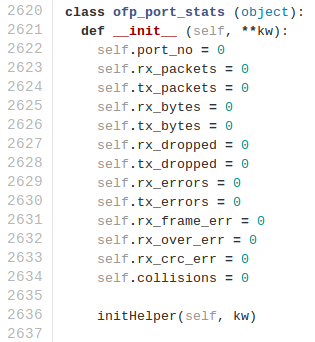
\includegraphics[width=0.8\textwidth]{figures/stats_portstats.png}
  \caption{Available port statistics}
  \label{fig:stats_portstats}
\end{minipage}%
\begin{minipage}{.5\textwidth}
  \centering
  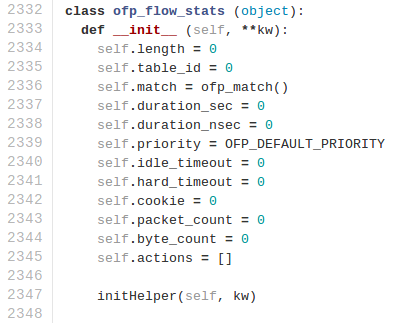
\includegraphics[width=1\textwidth]{figures/stats_flowstats.png}
  \caption{Available flow statistics}
  \label{fig:stats_flowstats}
\end{minipage}%
\end{figure}

Although a lot of port statistical values are available, bitrate is not one of them.
Without bitrate it is not possible to know the port usage ratio and as a consequence the switch usage ratio.
As this is a threat if one wants to develop an algorithm considering the network (\textit{e.g.} If network is considered for VM allocation, it makes no sense to allocate a VM in a server which is only connected to a overloaded switch).

Despite bitrate not being directly available, there are at least $2$ ways to obtain it.
One would be to change the OF switch implementation and protocol to implement it, but it is excessively intrusive and would turn the framework into a non standard option.
The other one would be to use the byte count (in and out) and a time counter. Although it is not an accurate solution, it is the most viable.

Respecting the statistics, POX implementation of the OF controller uses events for notifying that the statistics request is ready.
To obtain the bitrate as accurate as possible, a statistics request is made, the timestamp of the event with the statistical data is registered, a new request is made, and again the timestamp of the latest event is registered.
By subtracting the oldest timestamp to the newest it is obtained the time between the statistical data. The amount of bytes that were counted in that interval can be obtained in the same way. Finally by converting the bytes into bits (multiplying by $8$) and divide it by the time (converted to seconds), the bitrate is obtained.

\begin{verbatim}
#obtain the bit_rate for this port in mbps
bit_rate = ((bytes_count*8)/(time_elapsed))/1000000
\end{verbatim}

To calculate the port ratio the bitrate is divided by the port capacity. For the switch ratio, an average of all its ports ratios is made.
% warning, since now there is intervm communication, the way the switch ratio was being calculated is now wrong

Despite methods for accessing the statistics as they were collected is available, an alternative method is provided, which does a ponderation of the latest collected values with the average of the historical ones. The historical ponderation value can be changed in the configuration file.

\begin{verbatim}
bit_rate_port_stats[port_no] = 
        (self.historical_ponderation * temp_hist_bit_rate) + 
        ((1-self.historical_ponderation)* newest_bit_rate)

\end{verbatim}

Statistics can be collected, periodically (with periodicy indicated in the configuration file), can be retrieved whenever requested (\textit{e.g.} a VM request arrives) or both.

\subsubsection{Statistics Exporter}
\hspace{0.6cm}

\textit{Statistics Exporter} was created with the purpose of allowing statistics to be analyzed outside the running environment.
To do so, it periodically checks the \textit{statitics} module, collecting and saving all the information into '.csv' files.
\textit{Statistics exporter} should have the same periodicity for statistics collection than the \textit{statistics} module, in order to maximize the information gathered.
Two types of files are generated: for switches and for links.

\begin{figure}[h!tbp]
        \centering
        \includegraphics[width=0.7\textwidth]{figures/statsexport.png}
        \caption{Edge switch link statistics exported '.csv' file}
        \label{fig:statsexport}
\end{figure}

A link statistics file can be seen in figure \ref{fig:statsexport}. Columns represent the switch and its port, and lines the link ratio in each timestamp.
Where the files are saved can be chosen in the configuration file.

\subsection{VM Request Handler}
\hspace{0.6cm}

This module is responsible for parsing the VM requests (allocation or inter VM communication) and raising events with their requirements.
It creates a thread and a socket inside it for receiving and parsing the VM requests from both the \textit{VM Request Generator} and the \textit{WEB Platform}.
After the VM requests have been validated, an event with the VM requirements is raised.

For the VM allocation request the following event is raisen,

\begin{verbatim}
class VMRequest (Event) :
    '''
    Event with new virtual machine allocation request
    '''
    def __init__ (self, vm_id, time, cpu, ram, disk, 
                  network, request_type, timeout) :
        Event.__init__(self)
        self.vm_id = vm_id
        self.time = time
        self.cpu = cpu
        self.ram = ram
        self.disk = disk
        self.network = network
        self.request_type = request_type
        self.timeout = timeout
\end{verbatim}

Since inter VM communication is frequent in the DCs, allowing their communication without the need for the traffic to go to the gateway is important. For this reason, and because it is relevant that it is the administrator/network engineer defining the path, and event with the list of VMs to allow intercommunication is raised.

\begin{verbatim}
class InterVMComRequest (Event):
    """
    Event with the inter virtual machine communication request
    """
    def __init__(self, inter_vm_id, vm_list):
        Event.__init__(self)
        self.inter_vm_id = inter_vm_id
        self.vm_list = vm_list
\end{verbatim}

After the \textit{VMRequest} or the \textit{InterVMComRequest} have been processed and either allocated/accepted or rejected (typically in the \textit{User-defined logic}), this module communicates the state back to the source of the request.

\subsection{Network Traffic Requester}
\hspace{0.6cm}

The \textit{Network Traffic Requester} only function is to capture the event which says the VM as been allocated, and notify the mininet module \textit{Traffic Generator} to start generating traffic from the server in which the VM as been chosen to be allocated, with the network required characteristics and during the time the VM remains allocated

The network requirement varies according to the traffic generator being used, but in the case of \textit{Iperf}, just the amount of bandwidth is requested.

\subsection{VMM - Virtual Machines Manager}
\hspace{0.6cm}

This modules provides an abstraction level for the communication with the hypervisor. However, there are a lot of configurations that must be made before it can be used. These configurations vary from hypervisor to hypervisor, but in the case of \textit{XEN} are the installation of \textit{XCP} in each server, and the configuration of a VM template.

For the allocation process to be agile, a debian VM (other OSs are also supported) was previously installed and configured for external access. The idea is to clone this VM template, reducing the allocation time drastically.

By using XEN API, this process should not be hard to implement, however, what seemed like a simple implementation, rapidly became a ''nightmare'' since the available documentation is very poor, and there is a lack of examples.
With the impossibility of correctly interacting with \textit{Xen API}, a different approach was taken. By using ssh to control the machine where the hypervisor was installed, the \textit{xe} commands and a script created by citrix for cloning VM templates (can be seen in appendix \ref{app:clonevms}), a new VM was successfully allocated into a server.
When the VM gets allocated, it is automatically started up, and an IP addressed is given (this IP address which is later communicated to the sorce of the VM Request, so the VM can be accessed).

\subsection{User Defined Logic}
\label{subsec:userdeflog}
\hspace{0.6cm}

While all the other modules provide methods or data structures that ease the process of accessing and manipulating the information, this module just has to use those tools to produce the desired logic.
The \textit{User Define Logic} is a space for the administrators/network engineers to define their DC management policy (\textit{e.g.}VM allocation policies, smart DC routing, etc).
No limitations in terms of management functionalities are present. As long as everything is OF compliant and can be accessed through some provided API, it can be used in the logic.

Aiming to help the administrator/network engineer understanding in which ways it could be used, an hybrid VM allocation policy is included (takes into consideration the switches statistics and the server occupation), and also the Dijkstra algorithm is applied for calculating the shortest path between VMs that wish to communicate directly.

The hybrid VM allocation policy is fully described in \cite{im2013}. It includes $2$ algorithms for VM allocation: a server driven; and a network driven.

\begin{quotation}
''
a) Server-Driven algorithm

In the Server-Driven algorithm, first a physical server is selected for placing the VM, then a sequence of switches is chosen for forwarding the traffic flows to/from that VM across the DC network(...)\\

b) Network-Driven algorithm

In case of the Network-Driven algorithm, when a new VM placement request arrives, candidate core, aggregation and edge switches are firstly selected using a specific selection policy (e.g., FF, BF or WF) and checking that switches are able to process and forward the overall traffic possibly exchanged by the VM (i.e., the switches are not overloaded and at least one downlink is not congested) (...) Next, the physical server is selected within the set of servers directly connected to the candidate edge switch by applying a VM placement policy (e.g., FF, BF or WF) and checking that its network link is not congested (...) The VM placement process ends when the OF Controller inserts the proper forwarding rule in the edge, aggregation and core switches.''

\hfill Adami, D. et al.\cite{im2013}
\end{quotation}

With respect to the inter VM communication, an already implemented Dijkstra algorithm for shortest path was adopted (appendix \ref{app:dijkstra}). As the data structure for the topology (graph) was different, it had to be converted before calling the \textit{shortestpath} method. This method was used to calculate the shortest path between all combination of VM pairs.

The code for both implementations can be seen in \footnote{\url{https://github.com/jbteixeir/Openflow-DC-Framework/blob/master/ext/VM/vm\_allocation\_manager.py}. For allocation algorithms please check the methods \textit{networkDrivenAlgorithm} and \textit{serverDrivenAlgorithm}, and for inter VM communication \textit{interVMPathAlgorithm}}.

\subsection{Other POX Modules Used}
\hspace{0.6cm}

Besides using two POX modules on the topology module (\textit{Discovery} and \textit{host\_tracker}), another module was also used: dhcpd.
It is a simple DHCP server, which in the framework is used for attributing IP addresses for the newly created VMs.
For simplicity, all the parameters can be configured in the controllers configuration file.

\subsection{Configuration File}
\hspace{0.6cm}

The configuration file on the controller makes it easier to configure parameters that can easily change.
As one might prefer to insert the values in an interactive way, in case the configuration file does not exist, there is the possibility that each modules asks for the configuration it needs, and in the end it everything is written into a file.

\begin{minipage}{.5\textwidth}
  \begin{lstlisting}
[topology]
# link capacities in mbps
outside_link = 60
core_link = 60
agg_link = 30
edge_link = 10

[host]
#HOst Capacity
# cpu - number of cores
# Ram and Disk - GB
cpu = 8
ram = 16
disk = 2000

[hostippool]
#dhcpip - ip of the dhcp server
server=10.0.0.0/16
gateway=10.128.0.0/16
dhcpip=10.0.0.254
vm=10.128.128.0/24
dns=8.8.8.8

[stats]
# polling time - seconds
#Historial statistics weight
polling_time = 100
hist_weight = 0.125

[statsexport]
#directory where the switch and link statistics will be placed
switchsratiodir = ./stats
linksratiodir = ./stats
\end{lstlisting}
\end{minipage}%
\begin{minipage}{.5\textwidth}
    \begin{lstlisting}

[vmallocation]
# algorithms - ND/SD
#ND - Network Driven
#SD - Server Driven
algorithm = ND

# policies - FF/BF/WF
core_policy = BF
agg_policy = BF
edge_policy = BF
host_policy = BF

#maximum ratio a switch can have so it is chosen for new vm allocation
#maximum ratio a link can have so it is chosen for new vm allocation
switch_ratio = 1.20
link_ratio = 1.20

[vmreceiver]
#IP and port for listening to the VM requests
ip = 10.0.2.15
port = 3000

[credencial]
#Credential for xen hosts
username = root
password = xensource
\end{lstlisting}
\end{minipage}%

In the example above, the configuration file includes sections for the main framework modules, but as can be seen, a section for the VM allocation as been added, where it can be chosen which algorithms will be used, and even the maximum ratio for switches and links to still be considered when choosing the path.

Adding parameters is as simple as inserting them in the configuration file, and, in the module where they are used, assign them to variables.

\newpage

\section{Framework modules: Web Platform}
\hspace{0.6cm}

The \textit{WEB Platform} was created to provide the DC clients with a platform where their VM requests could be made and their VMs could be managed.

\subsection{Features and usage}
\hspace{0.6cm}

Although it still is an early development phase, the included features are:
\begin{itemize}
\item Authentication system for clients;
\item Request and View VMs;
\item Request and View VMs Groups (for inter VM communication);
\end{itemize}

\begin{figure}[h!tbp]
        \centering
        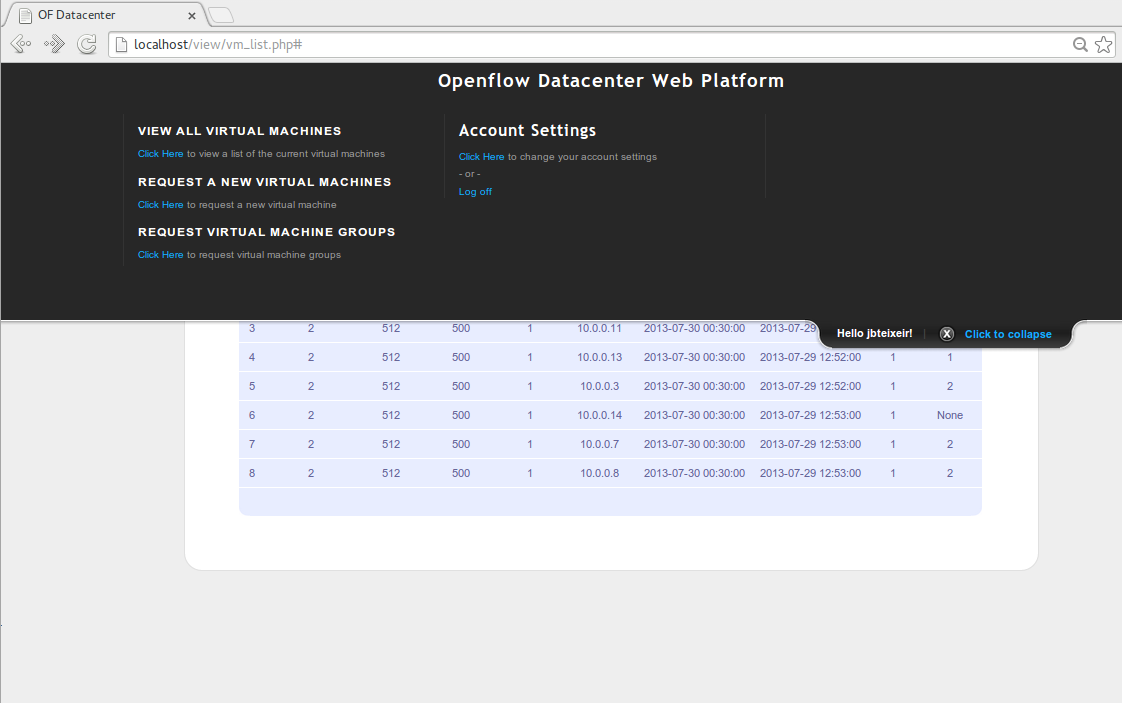
\includegraphics[width=1\textwidth]{figures/webplat_panel.png}
        \caption{WEB Platform - Top Panel}
        \label{fig:webplattop}
\end{figure}

The top panel of the WEB Platform is where the client can access all the available features, including to sign up or log in.
It can be seen in figure \ref{fig:webplattop}.

\begin{figure}[h!tbp]
        \centering
        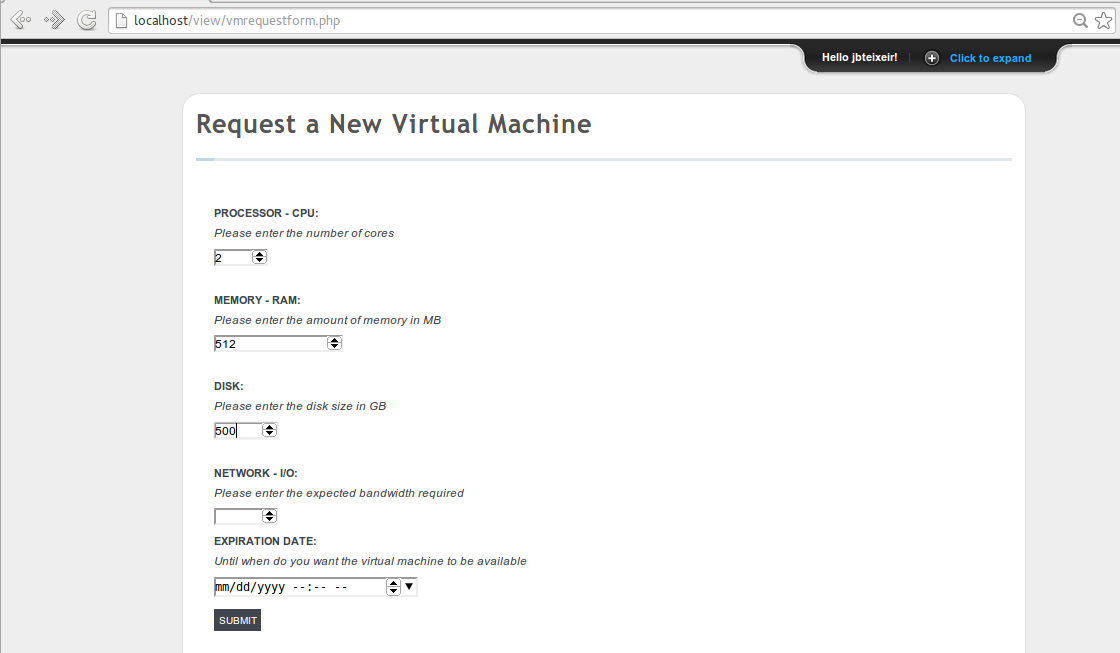
\includegraphics[width=1\textwidth]{figures/webplat_vmreq.png}
        \caption{WEB Platform - VM Request}
        \label{fig:webplatemreq}
\end{figure}

For requesting a VM the client needs to click in ''Request a new virtual machine'', fill the VM requirement fields and submit the request (figure \ref{fig:webplatemreq}). This request is sent to the controller, that after running the implemented allocation policy will install the rules and order the hypervisor to start the allocation process. When all these tasks are completed, the \textit{WEB Platform} is informed of the success state of the operation, and information for the VM to be accessed is returned.
If the client wants to view the VMs that it requested and their characteristics and current state, they are made available in ''View all virtual machines'' on the top panel (\ref{fig:webplatvmlist}).

\begin{figure}[h!tbp]
        \centering
        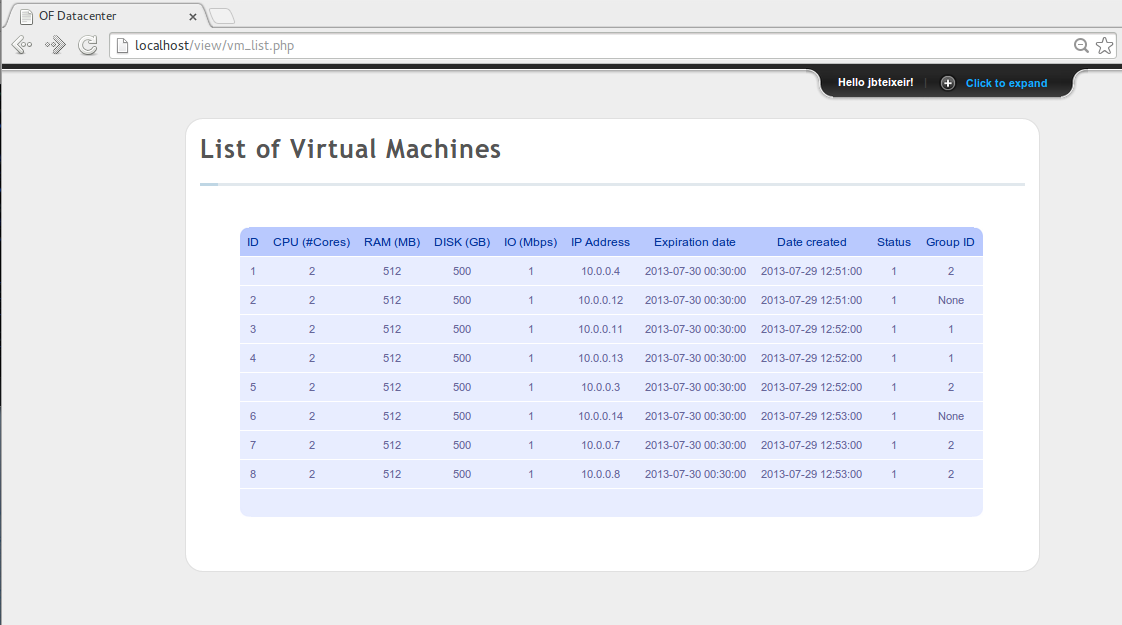
\includegraphics[width=1\textwidth]{figures/webplat_vmlist.png}
        \caption{WEB Platform - VM list}
        \label{fig:webplatvmlist}
\end{figure}

For requesting inter VM communication, a place for VM groups was created. The \textit{VM group} page as similar looks to the \textit{VM list} page, but with checkboxes for choosing the VMs that belong to the same group (figure \ref{fig:webplatvmgroup}).
After requesting a VM group, a similar process to the VM allocation request is started. Instead of running the allocation policy, the VM group policy is ran, the rules are installed and the feedback about the process is given back to the \textit{WEB Platform}.

\begin{figure}[h!tbp]
        \centering
        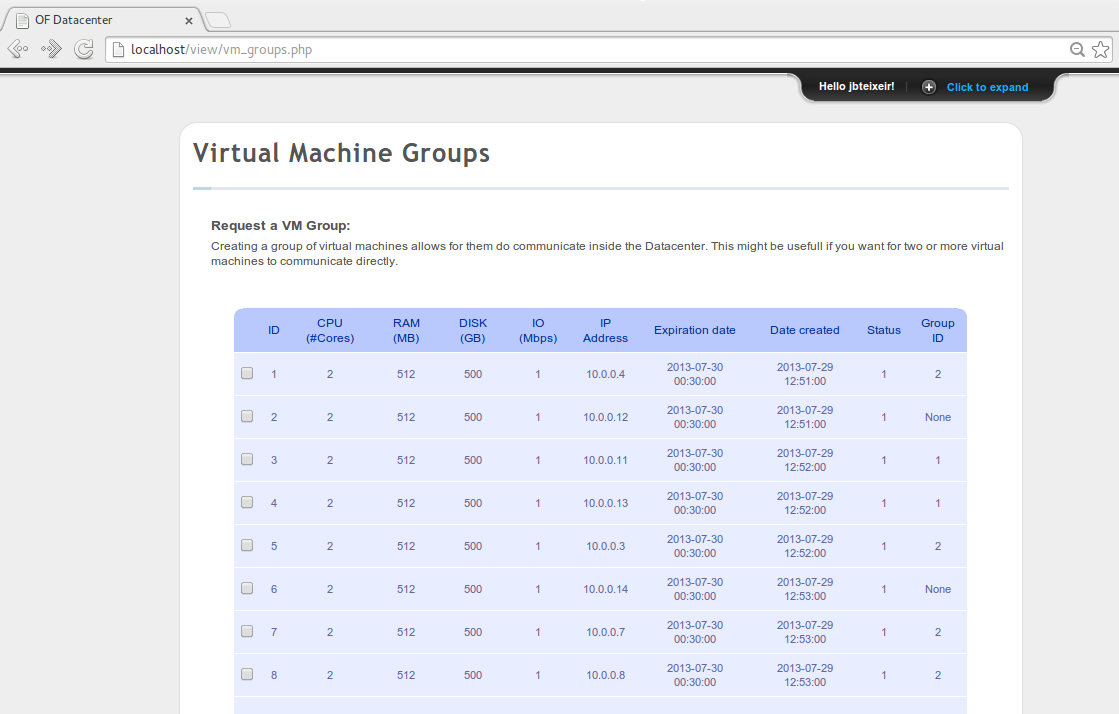
\includegraphics[width=1\textwidth]{figures/webplat_vmgroup.png}
        \caption{WEB Platform - VM Groups}
        \label{fig:webplatvmgroup}
\end{figure}

\newpage

\subsection{Design}
\hspace{0.6cm}

The architecture of the \textit{WEB Platform} follows the MVC (Model-view-controller) model.
It includes a MySql\cite{mysql} database to save information that is important for the \textit{WEB Platform} normal functioning. For now, most of the information is just a copy of the one kept by the OF controller. Security concerns are beyond this decision.
The database contains $3$ tables: ''users'' for keeping personal information about the users; ''vms'' for information related to the VMs (\textit{e.g} CPU, RAM, etc); and ''vm\_groups'' for mapping the VMs into the group they belong.
A script for creating this configuration can be seen in appendix \ref{app:mysql}.

For communicating with the OF controller a socket is opened and the requests are sent. For now they are string based requests, but it is planned to use an encrypted json\cite{JSON} notation.

\newpage
\section{Framework modules: VM Requester (VM Requests Generator)}
\hspace{0.6cm}

\begin{figure}[h!tbp]
        \centering
        \includegraphics[width=0.7\textwidth]{figures/vmreq.png}
        \caption{VM Requester console output}
        \label{fig:vmreq}
\end{figure}

As explained before, this modules is only to be used when testing. Its purpose is to automatically generate VM requests.
In order to do so, it uses a poisson random variable, for generating both the time interval between requests and the each of the requirements of the VM requests (CPU, RAM, DISK and Network).

Also developed in python, this independent program communicates with the controller \textit{VM request manager} to send VM requests.
It implements threads for receiving the status of the VM request, so it can at the same time keep making VM requests. The status are printed as the VMs get allocated.

\newpage

\section{Using the framework}

\subsection{Emulator}

\subsubsection{Setting up the development environment}
\hspace{0.6cm}

The mininet website provides a \textit{Ubuntu 12.04 LTS} virtual machine image with mininet (and all its dependencies) already installed and configured. By using this image in \textit{e.g} Virtualbox\cite{vbox} there is no need to change the native OS. If additionally ssh and ftp access to the Mininet VM are given, the administrator/network engineer can use its favorite text editor or IDE to change the code and test it.
For adding the framework to the Mininet VM, one just needs to copy the framework folder inside the VM.

\subsubsection{Testing new DC allocation policies}

The controller part of framework can be ran like a normal POX module. Its name is \textit{ercs}, and its responsible for calling all the submodules inside the controller. When testing, the \textit{DEBUG} log level should be activated, as it prints more information into the console.
\begin{verbatim}
~/poxbetta/pox.py ercs log.level --DEBUG
\end{verbatim}

For generating the desired topology, the configuration file provided under the same folder as the Mininet script must be changed, and script must be ran.
\begin{verbatim}
~/poxbetta/ext/Topology\ Generator\ \(MN\)/tpgeneratormn2.0.py 
\end{verbatim}

Finally, the VM requests are generated by running the following command,
\begin{verbatim}
python ~/poxbetta/ext/VM\ Requests\ Generator/vmrequesterpoisson.py {args}
\end{verbatim}

The list of arguments comprises the controller socket IP and port, the VM request rate and the VM requirements.

\newpage

In figure \ref{fig:emulenv} is a printscreen of all the components running.

\begin{figure}[h!tbp]
        \centering
        \includegraphics[width=1\textwidth]{figures/emulenv.png}
        \caption{Using the emulation environment. Top left: MN Topology Generator; Bottom left: VM Requests Generator; Right: Controller}
        \label{fig:emulenv}
\end{figure}

\newpage

\subsection{Real Environment}

\subsubsection{Setting up the real environment}
\hspace{0.6cm}

The real environment was assembled using real PCs for both the servers and the switches.
For the servers \textit{XCP 1.6} was used has the virtualization platform, and for the OF switches \textit{Open VSwitch - OF 1.0 complaint}, except for the ones that had NetFPGA cards\footnote{The NetFPGA is an open source hardware and software platform that is able to act as an OF 1.0 compliant switch}.

The implemented architecture is shown in figure \ref{fig:realenvarch}.

\begin{figure}[h!tbp]
        \centering
        \includegraphics[width=0.8\textwidth]{figures/realenvirscheme.png}
        \caption{Architecture of the real environment}
        \label{fig:realenvarch}
\end{figure}

Since OF separates the data plane from the control plane, two separate networks are required. Thus, a switch was added connecting the controller with all the OF switches.
For simplicity reasons, the laptop in the figure\ref{fig:realenvarch}, is simultaneously the gateway, the OF controller and the WEB Platform.

The specifications of the equipment used is shown below.
\begin{itemize}
  \item 2 x Servers
    \begin{itemize}
      \item Intel Xeon CPU 3075@2.66Ghz
      \item 4 GB Ram
      \item 900 GB HD
      \item NIC Intel 82566DM-2 Gigabit Network Connection
      \item NIC Intel 82541GI Gigabit Network Connection
    \end{itemize}
  \item 2 x Edge Switches and 2 x Aggregation Switches
    \begin{itemize}
      \item AMD Phenom 9650 Quad-Core \@ 1.16Ghz
      \item 450 GB HD
      \item 4 GiB RAM
      \item 2 x NIC Intel 82571EB Gigabit Ethernet Controller
      \item NIC Realtek Semiconductor RTL8111/8168B Pci Express Gigabit Ethernet Controller
    \end{itemize}

    \item 1 x Core Switch
    \begin{itemize}
      \item Intel Core i7 CPU 860 \@ 2.8Ghz x 8 
      \item 4 GiB Ram
      \item 450 GB HD
      \item NIC Realtek Semiconductor RTL8111/8168B Pci Express Gigabit Ethernet Controller
      \item NetFPGA 4 ports Gigabit Ethernet
    \end{itemize}

    \item 1 x Laptop (Gateway/Controller/WEB Platform)
    \begin{itemize}
      \item 1 Intel Core i5 2430M - 2.4Ghz x 4
      \item 8 GB RAM
      \item 500 GB HD
      \item 1 NIC Qualcomm Atheros AR8151 v2.0 Gigabit Ethernet
      \item 1 NIC Intel Corporation Centrino Wireless-N 100
      \item 1 NIC ASIX AX88772A USB 2.0 Fast Ethernet Network Adapter
    \end{itemize}
\end{itemize}

For enabling OF on the network interfaces of the non NetFPGA cards, a script was used. Although this configuration changes according to the network interfaces and their quantity, an example of the script can be found in appendix \ref{app:openvscript}.

Some problems where encountered while configuring the environment, namely: understanding why the controller was not able to connect the switches. Solved by creating a parallel network for the OF control plane; and network interfaces that were not detecting the network cable. Some network interfaces do not negotiate the link speed, so when some 100mbps NICs were connected to 1gbps NICs, they were not working. Solved by only connecting interfaces with the same link speed;

In figure \ref{fig:realenv}, a photo of the real environment is shown.

\begin{figure}[h!tbp]
        \centering
        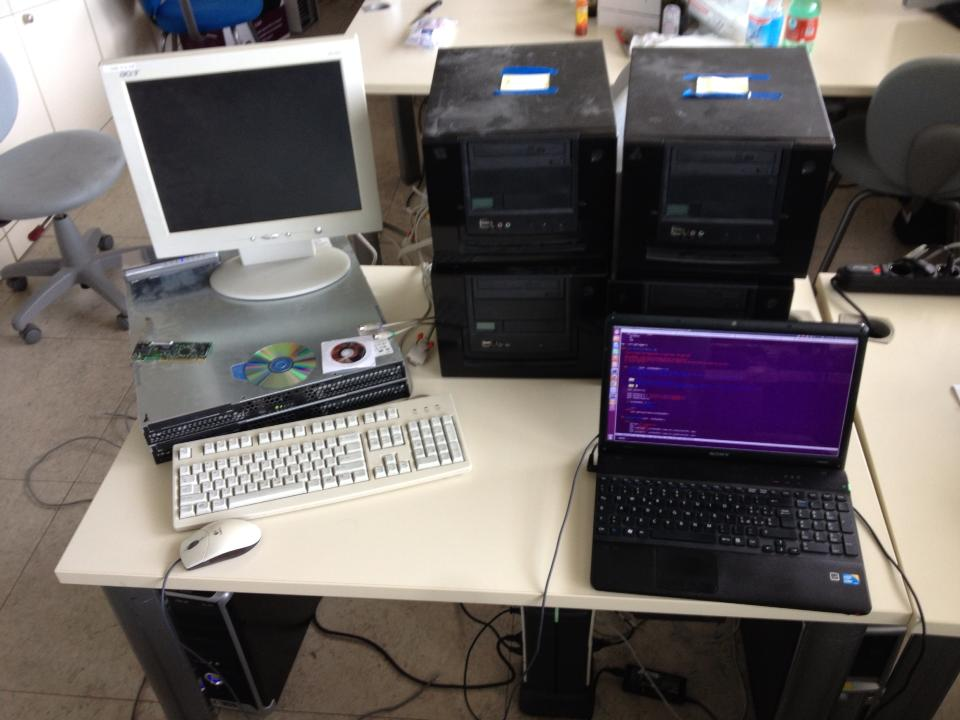
\includegraphics[width=0.8\textwidth]{figures/realenvironment.jpg}
        \caption{Photo of the testing environment. \textit{Table}: under the monitor - 2 servers; cube computer - aggregation and edge switches; laptop - DC gateway, controller and WEB Platform; \textit{Under the table}: core switch}
        \label{fig:realenv}
\end{figure}
\newpage

\section{Framework extensions \label{Sec:fraext} }
\hspace{0.6cm}

Framework extensions were though to allow a wider range of experiments and to show that important subjects are been taken into consideration. QoS and VM migration were the two chosen, one from the network side and the other from the IT resources.
As most of the framework, the extensions are still a work-in-progress, thus they should only be seen as experiments.

\subsection{Enabling QoS}
\subsubsection{State of art: QoS in Openflow}
\hspace{0.6cm}

The OF protocol as been evolving to provide support for QoS.
However, as they argue that will bring extra complexity \cite{qosof}, until version 1.3.1 (latest) they only added support for simple queuing mechanisms.
Version 1.0 started by bringing to queues minimum guaranteed rate but queue configuration was still done outside the OF protocol. Later, in version 1.2, maximum rate was also included.

Although this features are available most research efforts focus on QoS approaches to OF using, among other techniques, dynamic routing and are oriented for either streamming\cite{ofqos2}\cite{ofqos3} or multimedia\cite{ofqos1}.

Regarding mininet and its OF switches implementation, the latest version is 2.0 and contains Open VSwitch driver 1.3.4, which fully supports OF 1.0.
More recent versions of OF can be integrated by upgrading the version of Open VSwitch, however, they are still experimental and may not include all the features provided in the protocol specification.

\subsubsection{QoS in the framework}
\hspace{0.6cm}

As the framework aims for providing the administrators/network engineers the tools for developing and testing their logic, it is their responsibility to develop QoS tecniques/algorithms similar to the ones shown previously, while the framework should limit itself to help with the interaction with the OF supported QoS features and their expected usage in the cloud DC.

However, as an experiment, we went for a different perspective on how QoS is used.
It was implemented traffic differentiation for giving different type of user, different types of QoE.
Instead of following the traffic classes, it was created classes of users/VM types (\textit{e.g.} free users vs gold users; VoIP server vs web server vs etc), where each queue corresponds to a class.

Bringing QoS into the framework implied making changes in all the main modules, mostly because it is associated with the requests, and, as said before, the current implementation of queues in OF switches must be done manually.
The following modules where modified:
\begin{itemize}
  \item \textbf{Mininet Environment} -- Added to \textit{Topology Generator} a method for creating for each port in each switch, the number of desired queues (classes) and their corresponding percentage of the whole bandwidth. It also takes into consideration the different link's bandwidth. \textit{Dpctl} was the tool used for creating the queues and \textit{tc} for setting the minimum rate.

  \item \textbf{VM Requests Generator} -- Attached to VM Requests the type of class. The type of the VM request is chosen by the already existing poisson random variable.

  \item \textbf{Controller}
  \begin{itemize}
    \item \textbf{VM Request Manager} -- Changed requests parsing and events thrown to include type of class.
    \item \textbf{Rules} -- Created new methods for installing the rules that will send the flows to the specific queues. The main difference for the previous method was the action used: ''openflowlib.ofp\_action\_enqueue(port = switch\_port, queue\_id = queue\_type))'', which included not only the port where the packets should be forwarded, but also the queue.

    \item \textbf{VM Allocation Manager} -- This was modified just for performing tests (this is were the desired logic would be implemented).Changed algorithms to allocate each VM type to a corresponding servers. This helps checking if the tests work, since the OF protocol does not have statistics for queues, only for ports.
  \end{itemize}
\end{itemize}

Figure \ref{fig:ofqos} shows a representation of the mininet topology and how it was possible to test the QoS solution.
It started by creating the shown topology and setting the links bandwidth equal for edge-to-server links and edge-to-aggregation links (so the bandwidth would have to be disputed and it was possible to see the queues in action).
By allocating two VMs of different types into two servers that share the same edge switch, and by setting their IO requirements to the maximum bandwidth capacity of the edge-to-aggregation link that they share (first green link counting from the bottom), it should be possible to see the class with more "minimum rate" have at least the bandwidth corresponding to its class.
The minimum rate configuration for the classes was 70\%-30\%.

Unfortunately, by analysing the ratios of the blue and red links, it was not possible to see any differentiation. Both servers got half of the available bandwidth - an output that was not expected.

\begin{figure}[h!tbp]
        \centering
        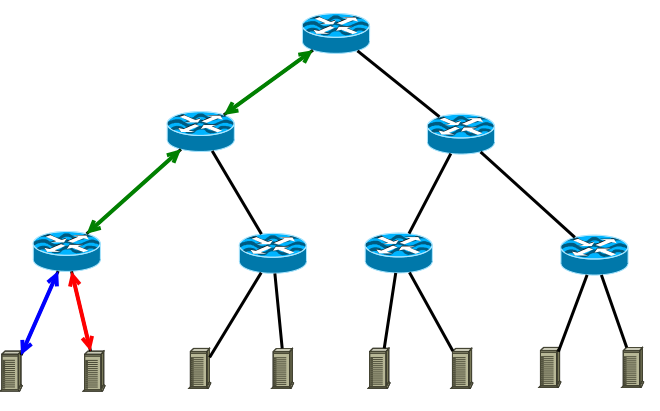
\includegraphics[width=0.8\textwidth]{figures/ofqos.png}
        \caption{QoS - Mininet testing environment}
        \label{fig:ofqos}
\end{figure}

A closer look to the article published online by the Openflow group\cite{qosof}, showed that the \textit{ENQUEUE} action was \textbf{not} supported yet, but that the queues could still be created and the flows could still be mapped to the queues by using the SET\_TOS and SET\_VLAN\_PCP OF parameters.
\begin{figure}[h!tbp]
        \centering
        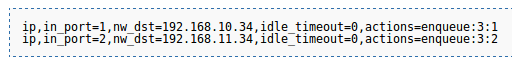
\includegraphics[width=0.8\textwidth]{figures/ofqosexample.png}
        \caption{QoS - Example of installed rules. Taken from \cite{qosof}}
        \label{fig:ofqosexample}
\end{figure}
As in their example they did not use any of these parameters, and the rules installed on the switches used the enqueue action (figure \ref{fig:ofqosexample}), the current implementation was misled.

\textit{Note: They have been contacted regarding how to reproduce such experiment, but no answer as been given yet.}

\newpage

\subsection{Enabling Virtual Machine migration}
\subsubsection{State of art: Virtual Machine migration}
\hspace{0.6cm}

VM migration is mostly handled by the hypervisors, which depending on the type of migration (live or not) take into consideration more or less requirements.
Research have been focus on helping making this tasks faster, simpler and without affecting the normal functioning of the DC.

More specifically, Stage A. et al. in \cite{vmmig1} discuss the management of bandwidth allocation while migrating VMs and also the assignment of priority to VM migration. They also propose an architecture design for DC.

Taking a step further, Boughzala, B. et al. \cite{vmmig2} used OF for supporting inter-domain VM migration. A study on how long rules take to be installed is made, and scalability is taken into consideration (usage of multiple OF controller, each with a specific OF domain). However it does not focus on helping VM migrations, only at allowing inter DCN migration.

By using OF rules to assist the Xen-based VM migration, Pedro S. Pisa et al \cite{vmmig3}, were able to have zero downtime. They also support WAN migration without packet loss due to the bilateral rule installation.

At last, Mishra, M. et al. in \cite{vmmig4}, present an overview of the VM migration techniques and how to use them to obtain dynamic resource management.
They point out the important characteristics of cloud-based DCs (Making resources available on demand, flexible resource provisioning and fine-grained metering), classify the resource management actions into types (server consolidation, load balancing and hotspot mitigation) and which heuristics are adopted (for each action) for answering when, which VM and where to migrate.

\subsubsection{Virtual Machine migration in the framework}
\hspace{0.6cm}

Aiming for providing full featured and generic access and control of the VM migration (being it live or not), a modified approach to the techniques previously presented was taken.

Although server consolidation and load balancing are the most used actions for resource management, they both fit in the same category - keeping DC policy.
Specially if we take into consideration the goal of the framework, it makes sense not to limit the resource management actions, but instead provide a generic way of keeping the DC policy, independently in what it is based (it might be server consolidation, but its up to the administrator/network engineer to define it).

\textit{Hotspot Mitigation} may also be split into server or network hotspot, which are quite different and have different ways of being solved.

Further more, since it is important to provide full access to DC, another question must be added -- which is the path chosen for VM migration.

For this to be possible, a few additions should be made to the controller:
\begin{itemize}
 \item Collect and save statistics from the servers.
 \item Add VM migration manager submodule to \textit{User-defined Logic}.
 \begin{itemize}
 \item \textit{When to migrate} -- Methods where it is defined how hotspots occurrence, for both network or server, are detected (or expected occurrence, so reactive and proactive VM migration are possible). Also a method for analyzing the current DC occupation (network and servers) and if it is not according to the defined policy (or combination of policies) start a VM migration process.
 \item \textit{Which VMs to migrate} -- Place for defining which VMs should be migrated.
 \item \textit{Where to migrate} -- Define where the VMs should be migrated.
 \item \textit{Which path to do the migration} -- Choose which path each migration should take.
 \end{itemize}
\end{itemize}

\newpage
Although all the above should be defined by the administrator/network engineer, it would be an advantage if it was possible to automatically manage the VMs so the logic defined for the allocation was kept over time. 
Meaning that, as time passes and VMs get allocated and deallocated, the way they are spread through the servers might not be the one which was previously defined.
\textit{E.g.} lets assume the best fit (server consolidation) algorithm is implemented and $2$ servers were full with VM allocations (6/6). If, after a while, half of the VMs in each server expire, instead of having just a server with all the VMs, we have two servers with half their capacity used -- table \ref{table:vmfrag}.

\begin{table}[h!tbp]
\centering
\begin{tabular}{c|c|c|}

\hline
\multicolumn{1}{|c|}{}& Server 1 & Server 2 \\
\hline
\multicolumn{1}{|c|}{When VMs were allocated} & 6/6 & 6/6 \\
\hline
\multicolumn{1}{|c|}{After some of them expired} & 3/6 & 3/6 \\
\hline
\hline
\multicolumn{1}{|c|}{What it should be if DC policy was kept (BF)} & 6/6 & 0/6 \\
\hline
\end{tabular}

\caption{DC servers occupation example. (VMs allocated / server VM allocation capacity)}
\label{table:vmfrag}
\end{table}

Having that in mind, but aiming for a generic way to keep any DC allocation logic over time, the following algorithm \ref{alg:keepdcpol} was developed.\\

\newpage
% \noindent\fbox{%
% \begin{varwidth}{\dimexpr\linewidth-2\fboxsep-2\fboxrule\relax}
\begin{algorithm}[h!]
\caption{Keep DC policy}
\label{alg:keepdcpol}
\begin{algorithmic}[1]
\State {\textit{\%retrieve the server list}}
\State {$server\_list\gets getServerList()$}
\State {\textit{\%retrieve server from the server list}}
\State {$server\gets getServerFromList(server\_list)$}
\While{$server \neq null$}
\State {\textit{\%retrieve the VM list}}
\State {$vm\_list\gets getVmList(server)$}
\State {\textit{\%retrieve vm from the VM list}}
\State {$vm\gets getVmFromList(vm\_list)$}
% \State{}
\While{$vm \neq null$}
\State {\textit{\%pretend to subtract the vm requirements to the server in which is allocated}}
\State {$subtractVmToDC(vm)$}
\State {\textit{\%run the user-defined policy to get the place where the vm would be allocated}}
\State {$new\_server \gets userDefinedAllocationPollicy(vm)$}
% \State{}
\If {$server \neq new\_server$}
\State {\textit{\%get the migration path for this vm}}
\State {$vm\_migration\_path \gets getVmMigrationPath(server, new\_server)$}
\State {\textit{\%start the vm migration}}
\State {$migrateVM(vm, server, new\_server, vm\_migration\_path)$}
\EndIf
% \State{}
\State {\textit{\%Remove this vm from the list}}
\State {$vm\_list\gets removeVmFromList(vm\_list, vm)$}
\State {\textit{\%retrieve other vm from the VM list}}
\State {$vm\gets getVmFromList(vm\_list)$}
\EndWhile

\State {\textit{\%Remove this server from the list}}
\State {$server\_list\gets removeServerFromList(server\_list, server)$}
\State {\textit{\%retrieve other server from the server list}}
\State {$server\gets getServerFromList(server\_list)$}
\EndWhile
\end{algorithmic}
\end{algorithm}
% \end{varwidth}% 
% }

The algorithm consists in, going to each server and each of its VMs and subtracting the VM requirements to the DC server in which it is allocated(so apparently the VM has not been allocated) and after run the user-defined VM allocation policy to see if it would change place.
If so, the path for migration is calculated, and the VM migration process starts.

For simplicity purpose, the algorithm took only into consideration the servers, but as it follows the same logic, the VM network path and other vm related aspects could also be included.

The algorithm as at least N complexity, but this varies as it must be multiplied by the complexity of the user-defined VM allocation algorithm and correspondent VM migration path calculation.

For analyzing the algorithms behaviour, two test were made using BF and WF.

\textit{Note: For the sake of simplicity, $3$ servers where taken into consideration with $3$ possible VM allocations, and all with the same requirements. The number of allocated VMs considered for the start of the algorithm was randomly generated (this set of numbers represents the state of the DC in a given time and results from the dynamics between the VM allocations and expirations. The order in which the VMs were chosen}

\begin{table}[h!tbp]
\begin{tabular}{lc|c|c||c|c|c|}
& \multicolumn{6}{c}{VM Allocation Policies} \\
\cline{2-7}
\multicolumn{1}{c|}{}& \multicolumn{3}{c||}{Best Fit} & \multicolumn{3}{c|}{Worst Fit} \\
\cline{2-7}
\multicolumn{1}{c|}{}& \multicolumn{3}{|c||}{Number of Virtual Machines}& \multicolumn{3}{c|}{Number of Virtual Machines} \\
\hline
\multicolumn{1}{|c|}{Iteration} & Server 1 & Server 2 & Server 3 & Server 1 & Server 2 & Server 3 \\
\hline
\multicolumn{1}{|c|}{Start} & 0 & 3 & 3 & 0 & 3 & 3 \\
\multicolumn{1}{|c|}{1} & 0 & 2 & 4 & 1 & 2 & 3 \\
\multicolumn{1}{|c|}{2} & 0 & 1 & 5 & 2 & 1 & 3 \\
\multicolumn{1}{|c|}{3} & 0 & 0 & 6 & 2 & 1 & 3 \\
\multicolumn{1}{|c|}{4} & 0 & 0 & 6 & 2 & 2 & 2 \\
\multicolumn{1}{|c|}{5} & 0 & 0 & 6 & 2 & 2 & 2 \\
\multicolumn{1}{|c|}{6} & 0 & 0 & 6 & 2 & 2 & 2 \\
\hline
\end{tabular}
\caption{Keep DC policy algorithm - Best Fit vs Worst Fit}
\label{table:keepdcpol}
\end{table}

Althought it is a very basic example, as can be seen in table \ref{table:keepdcpol}, the algorithm successfully recovered the DC policy.
On both cases, after the $3$rd iteration, no more migration were performed, however, as the algorithm runs through all the VMs, all $6$ iterations were made.

Although BF and WF do not, by far, represent all the types of VM allocation policies, they are a good starting point for the validation of the algorithm.
Further test should be made to ensure the algorithms correctiveness.
Assessing the efficiency and effective gain in the framework and real DC is yet to be made, but it is a point to be addressed in a near future.

-explain the goal of the keep dc policy
-explain better the tsarting opint of the example table
-explain the condition for choosing VMs
-take the on going part from the whole thesis
-trace statistics (average value, minimum and maxium levle of overall trafiic) time length peak traffic

\chapter{Validation and tests \label{cha:valtes} }

\section{Framework Validation}

Understanding the impact on the DC network infrastructure of well--known VM allocation policies represents the first step for finding more and more optimized solutions. The main concern was to validate th framework by analyzing the behaviour of the system under common situations, in order to compare the obtained results with the theoretical ones.

For this reason in the \textit{user-defined logic} part of the controller, it was firstly implemented Best Fit (BF), then Worst Fit (WF).
The BF algorithm chooses the server with the smallest available resources that still suits the requirements.
On the other hand WF chooses the one with the most available resources.
Therefore, it is expected that as each request comes, using a BF policy, all the VMs should be allocated in one single host until it is able to fulfill the requirements.
Then a new host will be selected, and so on until all the hosts have no more free space
 In the second case (\textit{i.e.}, WF policy), the VMs should be firstly equally spread through all 
the hosts.

The DC topology was configured with $1$ outside host, $2$ core switches, $4$ aggregation switches, $8$ edge switches, and $16$ hosts (\textit{i.e.}, $2$ per edge). Each host was configured to be able to allocate up to $3$ VM, for sake of simplicity (and to easily understand the results), and all the requests equal in terms of requirements (\textit{i.e.}, CPU, RAM, amount of disk space and bandwidth). It was defined the host (server) link ratio as the amount of traffic received per host (server) against the link speed set on the DC initialization phase. The DC was also configured in order to saturate the host link when three different VMs have been allocated.

\begin{figure}[h!tbp]
        \centering
        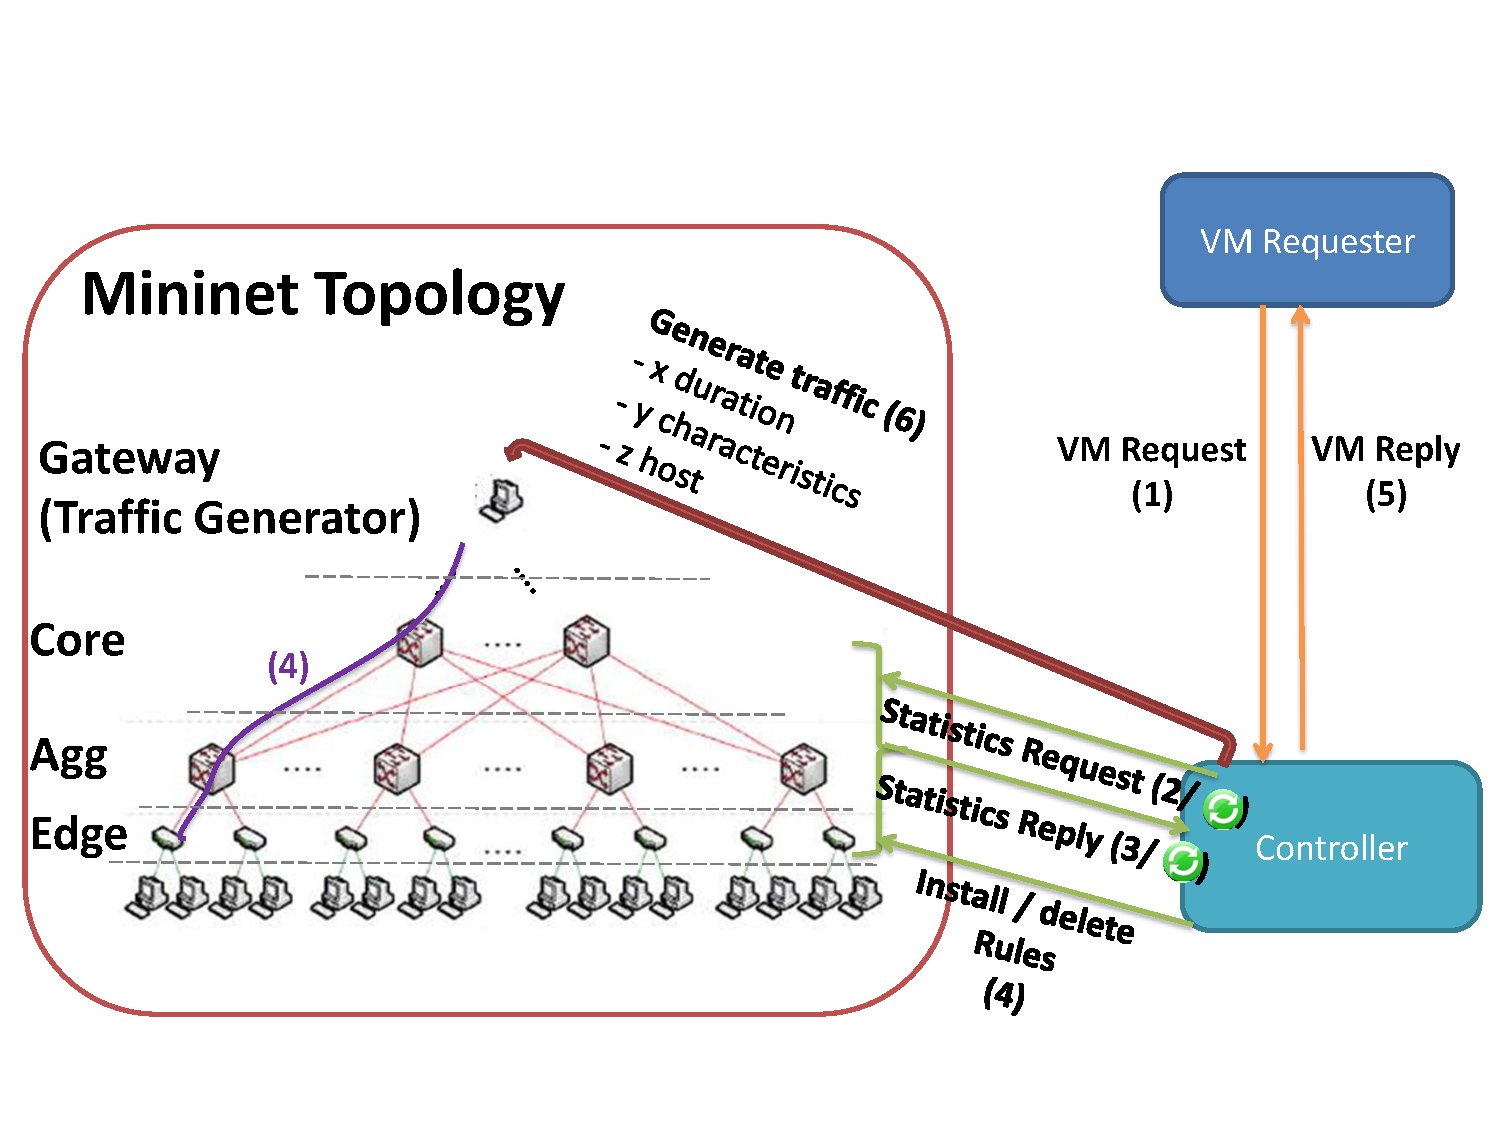
\includegraphics[width=0.8\textwidth]{figures/figure1.pdf}
        \caption{The environment}
        \label{fig:use_case}
\end{figure}


Figure \ref{fig:use_case} shows an high--level vision of the proposed environment. Starting from the framework, few lines of code were necessary to implement the allocation policy, since it provides all the necessary APIs to make sure that the controller can interact with the VM Requester, Traffic Generator and the DC switches.
Every time the controller receives a new VM allocation request (\textit{i.e.}, generated by the VM requester according to the DC configuration) it installs the proper rules on the switches (optionally it can ask for switches statistics -- even periodically). Once this process is completed, the controller informs the VM requester about the result of the allocation process and the traffic generation starts.


\begin{figure}[h!tbp]
        \centering
        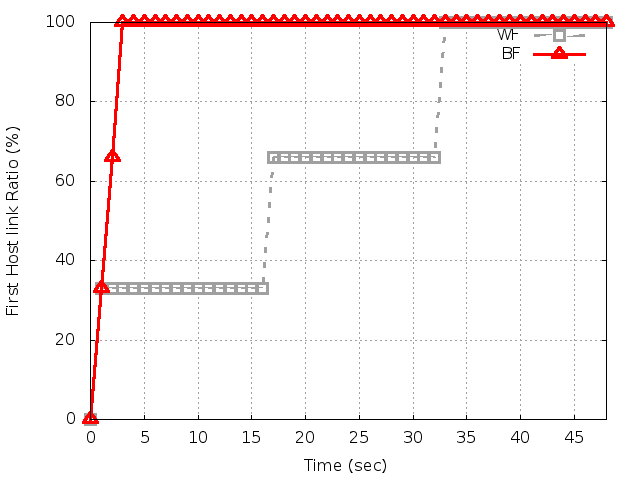
\includegraphics[width=0.6\textwidth]{figures/use_case.png}
        \caption{WF vs BF}
        \label{fig:wf_bf}
\end{figure}

Figure \ref{fig:wf_bf} shows the first host link ratio (link which connect the host to the edge switch) over the time.
Using a BF allocation policy, once a VM has been allocated in a host, all the following VMs are allocated in the same host until no more could be allocated (\textit{e.g.}, useful for energy saving). Having a new VM allocation request per second, after three seconds the first host link reaches the saturation.
Using the WF policy instead, the VMs should be firstly equally spread through all the hosts. In fact, being $16$ the DC hosts, and having just $1$ request per second, the first host link saturate at the $33$--th second.

\newpage

\section{Usecase: Hybrid VM Allocation policy}

For demonstrating the potential of combining the network and it resources management, and for showing that the framework is able to help doing it, the algorithms developed in \cite{im2013} were implemented and tested. The algorithms logic as already been explained previously on subsection \label{subsec:userdeflog}.

The results presented in the emulation part of \cite{im2013} were generated using this framework.

\begin{quotation}
''
b) Emulation results 
We tested our prototype directly on Mininet starting from a 3-
Tier DC network topology. We compared the switches utilization 
over the time with respect to the two joint it and network 
resources selection algorithms described in Section IV. 
Emulating a whole DC on Mininet by using a single machine 
requires too many HW resources. For this reason, we set-up a 
light DC environment where only a small number of switches 
was actually involved (i.e, 2 core switches, 8 aggregation 
switches and 16 edge switches) and where the link capacity 
between them was considerably scaled (i.e., from 1 Mbps to 10 
Mbps). In order to emulate the system behaviour we needed two 
more elements: 
\begin{itemize}
\item an agent in charge of actually perform the VM allocation 
requests; 
\item background traffic. 
\end{itemize}
The former is a script able to contact the OFVN controller 
asking for a VM with a given amount of CPU and traffic peak 
rate .VM allocation requests are generated according to a Poisson 
process whose inter-arrival time is exponentially distributed with an average $1/\lambda = 1$s.
We generated background traffic from a virtual host directly 
connected to the two Core switches. Finally, we set the mean 
value of the VM holding time to 85 minutes. 


\begin{figure}[h!tbp]
        \centering
        \includegraphics[width=1\textwidth]{figures/im2013graph.png}
        % \caption{\cite{im2013} Emulation Graphs}
        % \label{fig:wf_bf}
\end{figure}

Figures 18, 19 and 20 shows the mean switches utilization 
using the Server-driven algorithm. While the WF policy tries to 
spread as much as possible the load all over the switches the 
other two policies reveals to be less fair. For this reason, FF and 
BF policies could be mainly used when the energy saving is one 
of the main target of the system. In fact, such a non linear 
distribution in the switch selection process could be exploited to 
turn off some of the most unused switches. 

Figure 23 Core Switches Average Utilization -- Network-Driven Algorithm 
Figures 21, 22 and 23 shows the mean switches utilization 
using the Network-driven algorithm. In this case, it is worth 
highlighting a lower number of switches that are highly loaded. 
In fact, choosing the network path for first lead to privilege some 
switches with respect to others. Again, such policy is preferable 
when the energy saving is one of the main target of the system.
''
\hfill Adami, D. et al \cite{im2013}
\end{quotation}

\section{Performance Evaluation}
\label{sec:perf}
\hspace{0.6cm}

It was evaluated the actual performance of the proposed framework through a variety of experiments using a PC equipped with an Intel i5 3GHz and 8GB of DD3 RAM (\textit{i.e.}, from now on it will be called Host-PC).
The first tests have been carried out to inspect the impact of the amount of generated traffic, the DC topology size and the number of gateways on the server link ratio (from now on it will be called outside hosts to the gateways and hosts to the servers).
Firstly, it was generated a static topology (\textit{i.e}, $2$ outside hosts, $2$ core switches, $4$ aggregation switches, $8$ edge switches, $8$ hosts), then started up measuring the host link ratio increasing the generated traffic per host.

\begin{figure}[h!tbp]
        \centering
        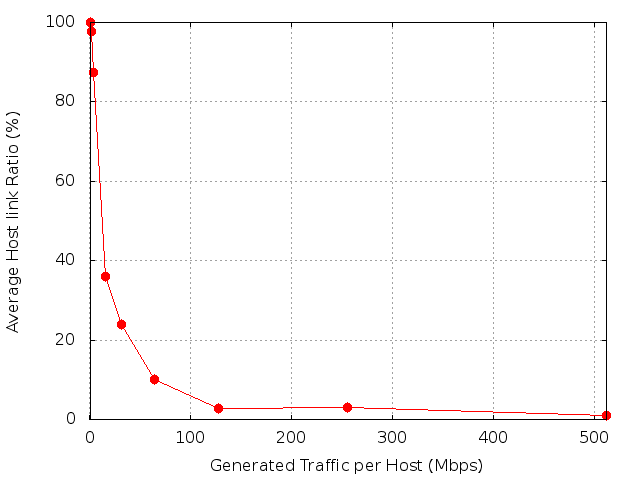
\includegraphics[width=0.7\textwidth]{figures/bw_utilization.png}
        \caption{Average Host link Ratio vs per Host Generated Traffic}
        \label{fig:bw}
\end{figure}

As shown in figure \ref{fig:bw} it was possible to generate up to few Mbps of traffic per host.
Then the host link ratio decreases as the generated traffic grows.
It is worth pointing out that such limitation does not affect any kind of DC performance tests made with the framework,
because the link speed can be scaled as much as wanted during the DC initialization phase, reaching every time 100\% of host link ratio.

In order to test the impact of the DC topology size on the
host link ratio the amount of the generated aggregated traffic was kept 
constant while exponentially increasing the number of switches and hosts.
The same testing topology was used.

On DC initialization phase, the link speed was configured in order to fully saturate the host links.

\begin{figure}[h!tbp]
        \centering
        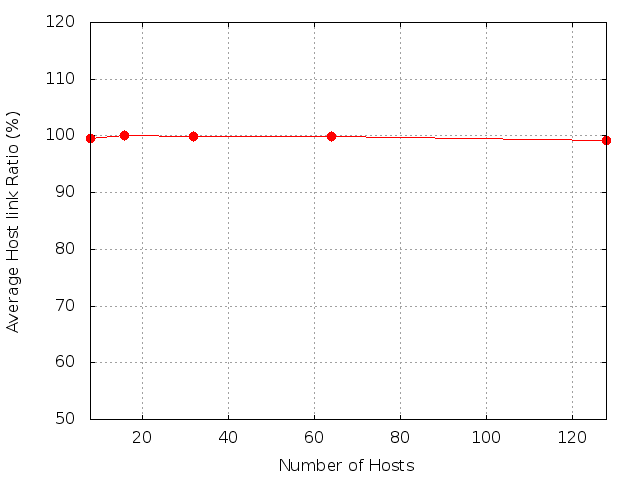
\includegraphics[width=0.7\textwidth]{figures/topo.png}
        \caption{Average Host Link Ratio vs number of Hosts}
        \label{fig:topo}
\end{figure}

The results in figure \ref{fig:topo} show that regardless of the hosts number, the host link ratio remains constant.
This means that as long as the total amount of generated traffic per host and the links speed can guarantee the link saturation, the system can scale indefinitely, being the only limits the Mininet itself, or the controller.

Finally it was investigated the relationship between the number of hosts connected to just one outside host and the average link ratio.

\newpage

\begin{figure}[h!tbp]
        \centering
        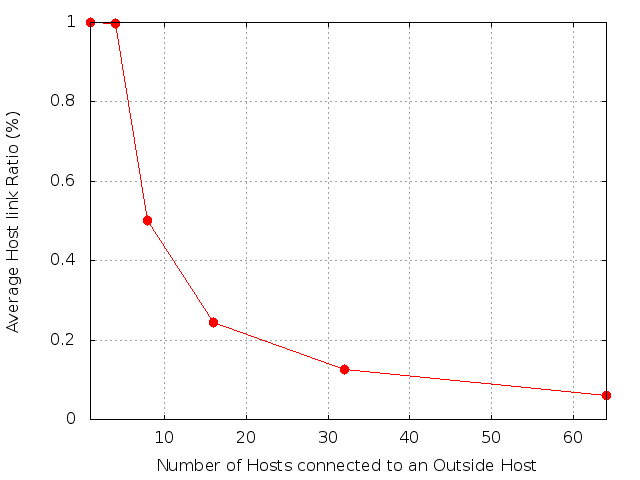
\includegraphics[width=0.7\textwidth]{figures/out_hosts_ratio.png}
        \caption{Average Host Link Ratio vs number of Hosts per Outside Host}
        \label{fig:hosts}
\end{figure}

Figure \ref{fig:hosts} shows that a maximum of $8$ hosts can be managed by just one outside host (\textit{i.e.}, the host link speed is set in order to have a link saturation).
Such a result gives to the user an important constraint that should be used during the DC configuration phase.
It is important to point out that this limitation is native of the Mininet environment and it is not due to our framework.

The second tests have been carried out to inspect the impact of both the amount of generated traffic and the DC topology size on the amount of memory the Host-PC needs.

\newpage

\begin{figure}[h!tbp]
        \centering
        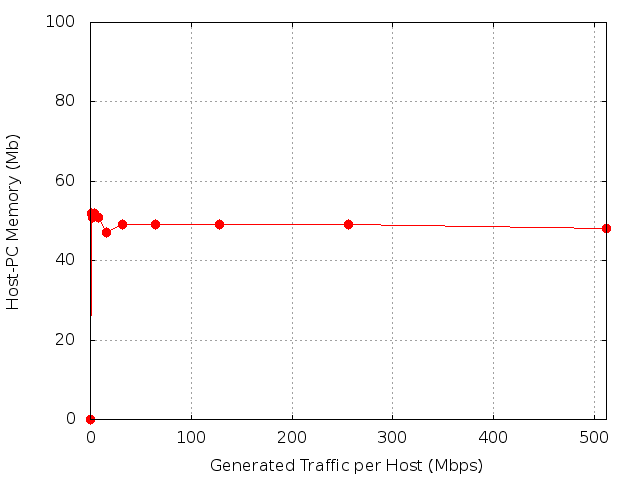
\includegraphics[width=0.7\textwidth]{figures/mem1_utilization.png}
        \caption{Host-PC Memory Utilization vs per Host Traffic Generated}
        \label{fig:mem1}
\end{figure}

\begin{figure}[h!tbp]
        \centering
        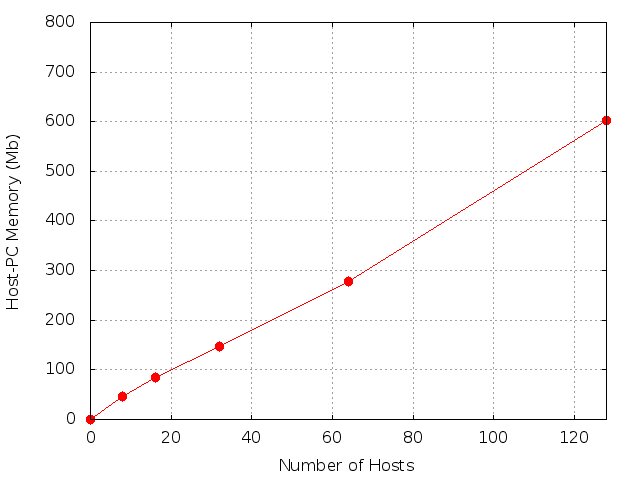
\includegraphics[width=0.7\textwidth]{figures/mem2_utilization.png}
        \caption{Host-PC Memory Utilization vs number of Hosts}
        \label{fig:mem2}
\end{figure}

Figure \ref{fig:mem1} shows that the memory utilization does not depend on the amount of generated traffic for each host.
On the other hand, as shown in figure \ref{fig:mem2}, as the topology size grows, the memory usage also grows in the same proportion, which allows to conclude that it scales linearly.
\newpage

\chapter{Conclusions\label{cha:conclusions}}
\hspace{0.6cm}

In this thesis, it was presented a novel SDN Cloud DC framework, built on top of Mininet and POX, that allows the DC administrator/network engineer to evaluate performances of their OF cloud DC controllers.
The framework addresses several issues in testing such controllers providing some useful APIs (i.e., topology discovery, traffic generation, DC configuration and VM request).
This work has been validated showing one use--case where two different well--known VMs scheduling algorithms were implemented.
Some of its potentials have also been demonstrated by implementing and testing VM hybrid policies.
Framework scalability and stability were also evaluated increasing both the number of emulated hosts and the DC links load. 

Openflow has been catching companies attention and gaining a lot of importance is a recent technology, however, as a new technology, a lot of features that usually can be seen on any router are still missing, which ends up limiting the features the framework makes available (\textit{e.g} regarding QoS).
Also, as a new technology, the existing controllers do not provide a lot of support, and solutions for encountered errors are not easily found or not found at all. For overcoming this errors, sometimes a deep knowledge of how the controller works is required.

A similar problem was faced when integrating \textit{XEN}, as the documentation is very poor, and few examples are available. This leds to conclude that even opensource projects that have success tend to neglect documentation.

Aiming to make the framework a more complete and mature solution, work is still in progress.

\section{Main contributions}
\hspace{0.6cm}

As a direct result of the work developed in this thesis, a contribution to the paper \textit{Virtualization-aware Network Control Strategies exploiting OpenFlow in Cloud Data Centers}\cite{im2013} emulation results was made.

Additionally, a paper focused only on the framework was created \textit{Datacenter in a box: test your SDN cloud-datacenter controller at home} and accepted into the EWSDN2013(Second European Workshop on Software Defined Networks)\cite{ewsdn}.


\section{Future work}

As an ongoing project, improvements can always be done, however, a few are already planned.

One would be to be able to access XEN through their API, since it would bring much more control and information over the servers and virtual machines.
The other would be to greatly improve the WEB Platform by not only giving the DC clients more information about their VMs and pricing tags but also to create a space for the DC administrator/network engineer to control and monitor the whole infrastructure.

\appendix

\chapter{Mininet Environment -- Configuration File\label{app:minconf}}

\begin{lstlisting}
Filename: conf.ini

[TopologySwitches]
#Integer value
#core_no - number of core switches
#agg_no - number of aggregation switches
#edge_no - number of edge switches
core_no = 4
agg_no = 8
edge_no = 16

[TopologyHosts]
#Integer value
#out_no - number of outside hosts
#host_no - number of hosts per edge switch
#host_detectacle_time - time in seconds in which the hosts send packets 
# so the host_tracker can detect them (0 == always detectable)
out_no = 4
host_no = 2
host_detectable_time = 2

[TopologyLinks]
#Integer value
#edgetoagglinkno - number of links that connect each edge switch to 
# aggregation switches
#aggtocorelinkno - number of links that connect each aggregation switch 
# to core switches
#coretooutlinkno - number of links that connect each core switch to 
# outside hosts
edgetoagglinkno = 2
aggtocorelinkno = 2
coretooutlinkno = 1

[SwitchBandwidth]
#Float value - mbps
#out_bw - bandwitdh for links that connect outside hosts
#core_bw - bandwitdh for links that connect core switches
#agg_bw - bandwitdh for links that connect aggregation switches
#edge_bw - bandwitdh for links that connect edge switches
out_bw = 4
core_bw = 4
agg_bw = 2
edge_bw = 1

[SwitchQueues]
#Float value
#queue_no - number of queues per switch and per port
#queue_number = bandwidth ratio - queue minimum bandwidth 
# (please use lower numbers for higher priority so the controller can assign premium users to this queues)  
queue_no = 2
queue_bw1 = 0.8
queue_bw2 = 0.2

[Traffic]
#Iperf configuration
#Amount of udp traffic against tcp one
#starting port for iperf to run on each host
udp_ratio = 0.5
iperf_port = 16000

\end{lstlisting}


\chapter{Mininet - DC Topology Generator Algorithm}
\label{app:tpalg}
\lstset{frame=tb,
  language=Python,
  aboveskip=3mm,
  belowskip=3mm,
  showstringspaces=false,
  columns=flexible,
  basicstyle={\small\ttfamily},
  numbers=none,
  numberstyle=\tiny\color{gray},
  keywordstyle=\color{blue},
  commentstyle=\color{dkgreen},
  stringstyle=\color{mauve},
  breaklines=true,
  breakatwhitespace=true
  tabsize=2
}


\begin{lstlisting}
    def generateTopology(self):
        #Out self.myhosts (self.myhosts that pretend to be the next thing after the gateway)
        for h in range(self.out_no):
            host_id = 'o%i'% (len(self.myhosts)+len(self.outside_hosts)+1)
            # Each outside host gets 30%/n of system CPU
            host = self.addHost(host_id)
            #host = self.addHost(host_id, cpu=0.5/((self.host_no*self.edge_no)+(self.out_no)))
            
            #set the ip of the outside host so it doesn't belong to the same subnet as the other hosts
            #TODO:net.getNodeByName(host).setIp("10.10.0."+str(h))

            #initialize link record
            self.alllinks[host_id] = list()
            
            #add host records
            self.outside_hosts.append(host_id)
                
        #Core Switches
        for s in range(self.core_no):
            switch_id = 'c%i'%(len(self.core_switches)+len(self.agg_switches)+len(self.edge_switches)+1)
            switch = self.addSwitch(switch_id)
            
            #Add edge switch records
            self.core_switches.append(switch_id)
            
            #initialize link records
            if not self.alllinks.has_key(switch_id):
                self.alllinks[switch_id] = list()
            
            #add link to out
            switch_link_no = 0
            self.outside_hosts.sort()
            for host_id in self.outside_hosts :
                if len(self.alllinks[host_id])<((self.core_no*self.core_out_link_no)/self.out_no):
                    self.addLink(switch_id, host_id, bw=self.out_bw)
                    #add link to record
                    self.alllinks[host_id].append(switch_id)
                    self.alllinks[switch_id].append(host_id)
                    switch_link_no += 1
                    
                if switch_link_no >= self.core_out_link_no:
                    break
            
            
             
            
        #Agg Switches
        for s in range(self.agg_no):
            switch_id = 'a%i'%(len(self.core_switches)+len(self.agg_switches)+len(self.edge_switches)+1)
            switch = self.addSwitch(switch_id)
            
            #Add edge switch records
            self.agg_switches.append(switch_id)
            
            #initialize link records
            if not self.alllinks.has_key(switch_id):
                self.alllinks[switch_id] = list()
            
            #TODO: add link to core
            switch_link_no = 0
            self.core_switches.sort()
            for core_id in self.core_switches :
                if len(self.alllinks[core_id])-self.core_out_link_no<((self.agg_no*self.agg_core_link_no)/self.core_no):
                    self.addLink(switch_id, core_id, bw = self.core_bw)
                    #add link to record
                    self.alllinks[core_id].append(switch_id)
                    self.alllinks[switch_id].append(core_id)
                    switch_link_no += 1
                    
                if switch_link_no >= self.agg_core_link_no:
                    break

                    
        #Edge Switches
        for s in range(self.edge_no):
            switch_id = 'e%i'%(len(self.core_switches)+len(self.agg_switches)+len(self.edge_switches)+1)
            switch = self.addSwitch(switch_id)
            
            #Add edge switch records
            self.edge_switches.append(switch_id)
            
            #initialize link records
            if not self.alllinks.has_key(switch_id):
                self.alllinks[switch_id] = list()
            
            #TODO: add link to agg
            switch_link_no = 0
            self.agg_switches.sort()
            for agg_id in self.agg_switches :
                if len(self.alllinks[agg_id])-self.agg_core_link_no<((self.edge_no*self.edge_agg_link_no)/self.agg_no):
                    mylink = self.addLink(switch_id, agg_id, bw = self.agg_bw)
                    #add link to record
                    self.alllinks[agg_id].append(switch_id)
                    self.alllinks[switch_id].append(agg_id)
                    switch_link_no += 1
                    
                if switch_link_no >= self.edge_agg_link_no:
                    break
            
            #add self.myhosts and connection to self.myhosts
            for h in range(self.host_no):
                host_id = 'h%i' % (len(self.myhosts)+len(self.outside_hosts)+1)
                # Each host gets 50%/n of system CPU
                host = self.addHost(host_id)
                #host = self.addHost(host_id, cpu=0.5/((self.host_no*self.edge_no)+(self.out_no)))
                
                #add link 100 Mbps, 5ms delay, 10% loss
                #self.addLink(host_id, switch_id, bw=10, delay='5ms', loss=10, max_queue_size=1000, use_htb=True
                self.addLink(host_id, switch_id, bw = self.edge_bw)
                
                #initialize link records
                if not self.alllinks.has_key(host_id):
                    self.alllinks[host_id] = list()
                    
                #add link records
                self.alllinks[host_id].append(switch_id)
                self.alllinks[switch_id].append(host_id)
                
                #add host records
                self.myhosts.append(host_id)
            
            #Add hosts until you can separate the host network and the outside host network
            len(self.myhosts)+len(self.outside_hosts)+1
\end{lstlisting}


\chapter{Sniffex.c Modified}
\label{app:sniffex}
\lstset{language=C,frame=lines}
\begin{lstlisting}
*
 * sniffex.c
 *
 * Sniffer example of TCP/IP packet capture using libpcap.
 * 
 * Version 0.1.1 (2005-07-05)
 * Copyright (c) 2005 The Tcpdump Group
 *
 * This software is intended to be used as a practical example and 
 * demonstration of the libpcap library; available at:
 * http://www.tcpdump.org/
 *
 ****************************************************************************
 *
 * This software is a modification of Tim Carstens' "sniffer.c"
 * demonstration source code, released as follows:
 * 
 * sniffer.c
 * Copyright (c) 2002 Tim Carstens
 * 2002-01-07
 * Demonstration of using libpcap
 * timcarst -at- yahoo -dot- com
 * 
 * "sniffer.c" is distributed under these terms:
 * 
 * Redistribution and use in source and binary forms, with or without
 * modification, are permitted provided that the following conditions
 * are met:
 * 1. Redistributions of source code must retain the above copyright
 *    notice, this list of conditions and the following disclaimer.
 * 2. Redistributions in binary form must reproduce the above copyright
 *    notice, this list of conditions and the following disclaimer in the
 *    documentation and/or other materials provided with the distribution.
 * 4. The name "Tim Carstens" may not be used to endorse or promote
 *    products derived from this software without prior written permission
 *
 * THIS SOFTWARE IS PROVIDED BY THE REGENTS AND CONTRIBUTORS ``AS IS'' AND
 * ANY EXPRESS OR IMPLIED WARRANTIES, INCLUDING, BUT NOT LIMITED TO, THE
 * IMPLIED WARRANTIES OF MERCHANTABILITY AND FITNESS FOR A PARTICULAR PURPOSE
 * ARE DISCLAIMED.  IN NO EVENT SHALL THE REGENTS OR CONTRIBUTORS BE LIABLE
 * FOR ANY DIRECT, INDIRECT, INCIDENTAL, SPECIAL, EXEMPLARY, OR CONSEQUENTIAL
 * DAMAGES (INCLUDING, BUT NOT LIMITED TO, PROCUREMENT OF SUBSTITUTE GOODS
 * OR SERVICES; LOSS OF USE, DATA, OR PROFITS; OR BUSINESS INTERRUPTION)
 * HOWEVER CAUSED AND ON ANY THEORY OF LIABILITY, WHETHER IN CONTRACT, STRICT
 * LIABILITY, OR TORT (INCLUDING NEGLIGENCE OR OTHERWISE) ARISING IN ANY WAY
 * OUT OF THE USE OF THIS SOFTWARE, EVEN IF ADVISED OF THE POSSIBILITY OF
 * SUCH DAMAGE.
 * <end of "sniffer.c" terms>
 *
 * This software, "sniffex.c", is a derivative work of "sniffer.c" and is
 * covered by the following terms:
 *
 * Redistribution and use in source and binary forms, with or without
 * modification, are permitted provided that the following conditions
 * are met:
 * 1. Because this is a derivative work, you must comply with the "sniffer.c"
 *    terms reproduced above.
 * 2. Redistributions of source code must retain the Tcpdump Group copyright
 *    notice at the top of this source file, this list of conditions and the
 *    following disclaimer.
 * 3. Redistributions in binary form must reproduce the above copyright
 *    notice, this list of conditions and the following disclaimer in the
 *    documentation and/or other materials provided with the distribution.
 * 4. The names "tcpdump" or "libpcap" may not be used to endorse or promote
 *    products derived from this software without prior written permission.
 *
 * THERE IS ABSOLUTELY NO WARRANTY FOR THIS PROGRAM.
 * BECAUSE THE PROGRAM IS LICENSED FREE OF CHARGE, THERE IS NO WARRANTY
 * FOR THE PROGRAM, TO THE EXTENT PERMITTED BY APPLICABLE LAW.  EXCEPT WHEN
 * OTHERWISE STATED IN WRITING THE COPYRIGHT HOLDERS AND/OR OTHER PARTIES
 * PROVIDE THE PROGRAM "AS IS" WITHOUT WARRANTY OF ANY KIND, EITHER EXPRESSED
 * OR IMPLIED, INCLUDING, BUT NOT LIMITED TO, THE IMPLIED WARRANTIES OF
 * MERCHANTABILITY AND FITNESS FOR A PARTICULAR PURPOSE.  THE ENTIRE RISK AS
 * TO THE QUALITY AND PERFORMANCE OF THE PROGRAM IS WITH YOU.  SHOULD THE
 * PROGRAM PROVE DEFECTIVE, YOU ASSUME THE COST OF ALL NECESSARY SERVICING,
 * REPAIR OR CORRECTION.
 * 
 * IN NO EVENT UNLESS REQUIRED BY APPLICABLE LAW OR AGREED TO IN WRITING
 * WILL ANY COPYRIGHT HOLDER, OR ANY OTHER PARTY WHO MAY MODIFY AND/OR
 * REDISTRIBUTE THE PROGRAM AS PERMITTED ABOVE, BE LIABLE TO YOU FOR DAMAGES,
 * INCLUDING ANY GENERAL, SPECIAL, INCIDENTAL OR CONSEQUENTIAL DAMAGES ARISING
 * OUT OF THE USE OR INABILITY TO USE THE PROGRAM (INCLUDING BUT NOT LIMITED
 * TO LOSS OF DATA OR DATA BEING RENDERED INACCURATE OR LOSSES SUSTAINED BY
 * YOU OR THIRD PARTIES OR A FAILURE OF THE PROGRAM TO OPERATE WITH ANY OTHER
 * PROGRAMS), EVEN IF SUCH HOLDER OR OTHER PARTY HAS BEEN ADVISED OF THE
 * POSSIBILITY OF SUCH DAMAGES.
 * <end of "sniffex.c" terms>
 * 
 ****************************************************************************
 *
 * Below is an excerpt from an email from Guy Harris on the tcpdump-workers
 * mail list when someone asked, "How do I get the length of the TCP
 * payload?" Guy Harris' slightly snipped response (edited by him to
 * speak of the IPv4 header length and TCP data offset without referring
 * to bitfield structure members) is reproduced below:
 * 
 * The Ethernet size is always 14 bytes.
 * 
 * <snip>...</snip>
 *
 * In fact, you *MUST* assume the Ethernet header is 14 bytes, *and*, if 
 * you're using structures, you must use structures where the members 
 * always have the same size on all platforms, because the sizes of the 
 * fields in Ethernet - and IP, and TCP, and... - headers are defined by 
 * the protocol specification, not by the way a particular platform's C 
 * compiler works.)
 *
 * The IP header size, in bytes, is the value of the IP header length,
 * as extracted from the "ip_vhl" field of "struct sniff_ip" with
 * the "IP_HL()" macro, times 4 ("times 4" because it's in units of
 * 4-byte words).  If that value is less than 20 - i.e., if the value
 * extracted with "IP_HL()" is less than 5 - you have a malformed
 * IP datagram.
 *
 * The TCP header size, in bytes, is the value of the TCP data offset,
 * as extracted from the "th_offx2" field of "struct sniff_tcp" with
 * the "TH_OFF()" macro, times 4 (for the same reason - 4-byte words).
 * If that value is less than 20 - i.e., if the value extracted with
 * "TH_OFF()" is less than 5 - you have a malformed TCP segment.
 *
 * So, to find the IP header in an Ethernet packet, look 14 bytes after 
 * the beginning of the packet data.  To find the TCP header, look 
 * "IP_HL(ip)*4" bytes after the beginning of the IP header.  To find the
 * TCP payload, look "TH_OFF(tcp)*4" bytes after the beginning of the TCP
 * header.
 * 
 * To find out how much payload there is:
 *
 * Take the IP *total* length field - "ip_len" in "struct sniff_ip" 
 * - and, first, check whether it's less than "IP_HL(ip)*4" (after
 * you've checked whether "IP_HL(ip)" is >= 5).  If it is, you have
 * a malformed IP datagram.
 *
 * Otherwise, subtract "IP_HL(ip)*4" from it; that gives you the length
 * of the TCP segment, including the TCP header.  If that's less than
 * "TH_OFF(tcp)*4" (after you've checked whether "TH_OFF(tcp)" is >= 5),
 * you have a malformed TCP segment.
 *
 * Otherwise, subtract "TH_OFF(tcp)*4" from it; that gives you the
 * length of the TCP payload.
 *
 * Note that you also need to make sure that you don't go past the end 
 * of the captured data in the packet - you might, for example, have a 
 * 15-byte Ethernet packet that claims to contain an IP datagram, but if 
 * it's 15 bytes, it has only one byte of Ethernet payload, which is too 
 * small for an IP header.  The length of the captured data is given in 
 * the "caplen" field in the "struct pcap_pkthdr"; it might be less than 
 * the length of the packet, if you're capturing with a snapshot length 
 * other than a value >= the maximum packet size.
 * <end of response>
 * 
 ****************************************************************************
 * 
 * Example compiler command-line for GCC:
 *   gcc -Wall -o sniffex sniffex.c -lpcap
 * 
 ****************************************************************************
 *
 * Code Comments
 *
 * This section contains additional information and explanations regarding
 * comments in the source code. It serves as documentaion and rationale
 * for why the code is written as it is without hindering readability, as it
 * might if it were placed along with the actual code inline. References in
 * the code appear as footnote notation (e.g. [1]).
 *
 * 1. Ethernet headers are always exactly 14 bytes, so we define this
 * explicitly with "#define". Since some compilers might pad structures to a
 * multiple of 4 bytes - some versions of GCC for ARM may do this -
 * "sizeof (struct sniff_ethernet)" isn't used.
 * 
 * 2. Check the link-layer type of the device that's being opened to make
 * sure it's Ethernet, since that's all we handle in this example. Other
 * link-layer types may have different length headers (see [1]).
 *
 * 3. This is the filter expression that tells libpcap which packets we're
 * interested in (i.e. which packets to capture). Since this source example
 * focuses on IP and TCP, we use the expression "ip", so we know we'll only
 * encounter IP packets. The capture filter syntax, along with some
 * examples, is documented in the tcpdump man page under "expression."
 * Below are a few simple examples:
 *
 * Expression     Description
 * ----------     -----------
 * ip         Capture all IP packets.
 * tcp          Capture only TCP packets.
 * tcp port 80      Capture only TCP packets with a port equal to 80.
 * ip host 10.1.2.3   Capture all IP packets to or from host 10.1.2.3.
 *
 ****************************************************************************
 *
 */

#define APP_NAME    "sniffex"
#define APP_DESC    "Sniffer example using libpcap"
#define APP_COPYRIGHT "Copyright (c) 2005 The Tcpdump Group"
#define APP_DISCLAIMER  "THERE IS ABSOLUTELY NO WARRANTY FOR THIS PROGRAM."

#include <pcap.h>
#include <stdio.h>
#include <string.h>
#include <stdlib.h>
#include <ctype.h>
#include <errno.h>
#include <sys/types.h>
#include <sys/socket.h>
#include <netinet/in.h>
#include <netinet/ip.h>
#include <arpa/inet.h>
#include <unistd.h>
#include <signal.h>
#include <byteswap.h>
#include <math.h>
#include <errno.h>

#define min(a,b) ( (a) < (b) ? (a) : (b) )
#define SR_PACKET_DUMP_SIZE 1514
#define DEFAULT_IFACE "nf2c0"

/*Handle arguments*/
int c;
char *logfile = NULL;
char *interface = NULL;
char *filename = NULL;
pcap_dumper_t* file;

char *dev = NULL;         /* capture device name */
pcap_t *handle;           /* packet capture handle */
bpf_u_int32 mask;         /* subnet mask */
bpf_u_int32 net;          /* ip */
char errbuf[PCAP_ERRBUF_SIZE];    /* error buffer */

char ipSourceAddressString[16] = "";
char ipDestAddressString[16] = "";


/* default snap length (maximum bytes per packet to capture) */
#define SNAP_LEN 1518

/* ethernet headers are always exactly 14 bytes [1] */
#define SIZE_ETHERNET 14

/* Ethernet addresses are 6 bytes */
#define ETHER_ADDR_LEN  6

/* Ethernet header */
struct sniff_ethernet {
        u_char  ether_dhost[ETHER_ADDR_LEN];    /* destination host address */
        u_char  ether_shost[ETHER_ADDR_LEN];    /* source host address */
        u_short ether_type;                     /* IP? ARP? RARP? etc */
};

/* IP header */
struct sniff_ip {
        u_char  ip_vhl;                 /* version << 4 | header length >> 2 */
        u_char  ip_tos;                 /* type of service */
        u_short ip_len;                 /* total length */
        u_short ip_id;                  /* identification */
        u_short ip_off;                 /* fragment offset field */
        #define IP_RF 0x8000            /* reserved fragment flag */
        #define IP_DF 0x4000            /* dont fragment flag */
        #define IP_MF 0x2000            /* more fragments flag */
        #define IP_OFFMASK 0x1fff       /* mask for fragmenting bits */
        u_char  ip_ttl;                 /* time to live */
        u_char  ip_p;                   /* protocol */
        u_short ip_sum;                 /* checksum */
        struct  in_addr ip_src,ip_dst;  /* source and dest address */
};

#define IP_HL(ip)               (((ip)->ip_vhl) & 0x0f)
#define IP_V(ip)                (((ip)->ip_vhl) >> 4)

/* TCP header */
typedef u_int tcp_seq;

struct sniff_tcp {
        u_short th_sport;               /* source port */
        u_short th_dport;               /* destination port */
        tcp_seq th_seq;                 /* sequence number */
        tcp_seq th_ack;                 /* acknowledgement number */
        u_char  th_offx2;               /* data offset, rsvd */
#define TH_OFF(th)      (((th)->th_offx2 & 0xf0) >> 4)
        u_char  th_flags;
        #define TH_FIN  0x01
        #define TH_SYN  0x02
        #define TH_RST  0x04
        #define TH_PUSH 0x08
        #define TH_ACK  0x10
        #define TH_URG  0x20
        #define TH_ECE  0x40
        #define TH_CWR  0x80
        #define TH_FLAGS        (TH_FIN|TH_SYN|TH_RST|TH_ACK|TH_URG|TH_ECE|TH_CWR)
        u_short th_win;                 /* window */
        u_short th_sum;                 /* checksum */
        u_short th_urp;                 /* urgent pointer */
};

void
print_payload(const u_char *payload, int len);

void
print_hex_ascii_line(const u_char *payload, int len, int offset);

void
print_app_banner(void);

void
print_app_usage(void);

/*
 * app name/banner
 */
void
print_app_banner(void)
{

  printf("%s - %s\n", APP_NAME, APP_DESC);
  printf("%s\n", APP_COPYRIGHT);
  printf("%s\n", APP_DISCLAIMER);
  printf("\n");

return;
}

/*
 * print help text
 */
void
print_app_usage(void)
{

  printf("Usage: %s [interface]\n", APP_NAME);
  printf("\n");
  printf("Options:\n");
  printf("    interface    Listen on <interface> for packets.\n");
  printf("\n");

return;
}

/*
 * print data in rows of 16 bytes: offset   hex   ascii
 *
 * 00000   47 45 54 20 2f 20 48 54  54 50 2f 31 2e 31 0d 0a   GET / HTTP/1.1..
 */
void
print_hex_ascii_line(const u_char *payload, int len, int offset)
{

  int i;
  int gap;
  const u_char *ch;

  /* offset */
  printf("%05d   ", offset);
  
  /* hex */
  ch = payload;
  for(i = 0; i < len; i++) {
    printf("%02x ", *ch);
    ch++;
    /* print extra space after 8th byte for visual aid */
    if (i == 7)
      printf(" ");
  }
  /* print space to handle line less than 8 bytes */
  if (len < 8)
    printf(" ");
  
  /* fill hex gap with spaces if not full line */
  if (len < 16) {
    gap = 16 - len;
    for (i = 0; i < gap; i++) {
      printf("   ");
    }
  }
  printf("   ");
  
  /* ascii (if printable) */
  ch = payload;
  for(i = 0; i < len; i++) {
    if (isprint(*ch))
      printf("%c", *ch);
    else
      printf(".");
    ch++;
  }

  printf("\n");

return;
}

/*
 * print packet payload data (avoid printing binary data)
 */
void
print_payload(const u_char *payload, int len)
{

  int len_rem = len;
  int line_width = 16;      /* number of bytes per line */
  int line_len;
  int offset = 0;         /* zero-based offset counter */
  const u_char *ch = payload;

  if (len <= 0)
    return;

  /* data fits on one line */
  if (len <= line_width) {
    print_hex_ascii_line(ch, len, offset);
    return;
  }

  /* data spans multiple lines */
  for ( ;; ) {
    /* compute current line length */
    line_len = line_width % len_rem;
    /* print line */
    print_hex_ascii_line(ch, line_len, offset);
    /* compute total remaining */
    len_rem = len_rem - line_len;
    /* shift pointer to remaining bytes to print */
    ch = ch + line_len;
    /* add offset */
    offset = offset + line_width;
    /* check if we have line width chars or less */
    if (len_rem <= line_width) {
      /* print last line and get out */
      print_hex_ascii_line(ch, len_rem, offset);
      break;
    }
  }

return;
}

uint16_t do_cksum(uint16_t *addr, int len)
{
    int nleft = len;
    uint16_t *w = addr;
    uint16_t answer;
    uint32_t sum = 0;

    /*
     *  Our algorithm is simple, using a 32 bit accumulator (sum),
     *  we add sequential 16 bit words to it, and at the end, fold
     *  back all the carry bits from the top 16 bits into the lower
     *  16 bits.
     */
    while (nleft > 1)  {
        sum += ntohs(*w++);
        nleft -= 2;
    }

    /* mop up an odd byte, if necessary */
    if (nleft == 1){
        sum += *(reinterpret_cast<u_char *>(w));
    }

    /*
     * add back carry outs from top 16 bits to low 16 bits
     */
    sum = (sum >> 16) + (sum & 0xffff); /* add hi 16 to low 16 */
    sum += (sum >> 16);         /* add carry */
    answer = ~sum;              /* truncate to 16 bits */
    return (answer);
}

void ex_programm(int sig){
    pcap_dump_close(file);
    (void)signal(SIGINT, SIG_DFL);
}

void pcap_spoof_ip(unsigned char* arg, const struct pcap_pkthdr * pkt_hdr, unsigned char const* packet) {
    
  struct pcap_pkthdr h;
  int size;
    int len;
    int i;
    int size_ip;
    unsigned char s_octet[4] = {0,0,0,0};
    unsigned char d_octet[4] = {0,0,0,0};
    
    /* declare pointers to packet headers */
  const struct sniff_ethernet *ethernet;  /* The ethernet header [1] */
  struct sniff_ip *ip;              /* The IP header */
    
    (void)signal(SIGINT,ex_programm);
 
  /* Get info from packet header */
    len = pkt_hdr->caplen;
    size = min(SR_PACKET_DUMP_SIZE, len);
    
    /* Copy packet */
    unsigned char* packet_cpy;
  packet_cpy = (unsigned char*) malloc(len);
  memcpy(packet_cpy, packet, len);
    
    ethernet = (const struct sniff_ethernet *)packet;
    
    uint16_t ether_type = ntohs(ethernet->ether_type);
    
    /* Remake IP Addresses on the copied packet */
    if(ether_type == 0x0800)
    ip = (struct sniff_ip*)(packet_cpy+SIZE_ETHERNET);
  else if(ether_type == 0x8100)
    ip = (struct sniff_ip*)(packet_cpy+SIZE_ETHERNET+4);
    
    ip->ip_ttl = 14;
    
    size_ip = IP_HL(ip)*4;
  if (size_ip < 20) {
    printf("* Invalid IP header length: %u bytes\n", size_ip);
    return;
  }
  
    
    in_addr *new_s;
    new_s = (in_addr*) malloc(sizeof(struct in_addr));
    
    
    in_addr *new_d;
    new_d = (in_addr*) malloc(sizeof(struct in_addr));
    
    inet_aton(ipSourceAddressString,  new_s);
    ip->ip_src = *new_s;
  
  inet_aton(ipDestAddressString,  new_d);
    ip->ip_dst = *new_d;
    
    /* For Debug Purposes
  ip->saddr = ntohl(new_saddr);
    ip->daddr = ntohl(new_daddr);
    
    for (i=0; i<4; i++)
  s_octet[i] = (ip->saddr >>(i*8)) & 0xFF;

    for (i=0; i<4; i++)
        d_octet[i] = (ip->daddr >>(i*8)) & 0xFF;
        
  printf("NEW source ip: %d.%d.%d.%d\n",s_octet[3],s_octet[2],s_octet[1],s_octet[0]);
    printf("NEW destination ip: %d.%d.%d.%d\n",d_octet[3],d_octet[2],d_octet[1],d_octet[0]);
  */
  
  /* Recalculate Checksum */
  ip->ip_sum=0;
  uint16_t new_cksm = 0;
  if(ether_type == 0x0800)
    new_cksm=do_cksum(reinterpret_cast<uint16_t*>(packet_cpy+SIZE_ETHERNET),sizeof(struct sniff_ip));
  else if(ether_type == 0x8100)
    new_cksm=do_cksum(reinterpret_cast<uint16_t*>(packet_cpy+SIZE_ETHERNET+4),sizeof(struct sniff_ip));
    ip->ip_sum=htons(new_cksm);
    
    
    /* Dump the packet */    
    //h.caplen = pkt_hdr->caplen;
    //h.len = (size < SR_PACKET_DUMP_SIZE) ? size : SR_PACKET_DUMP_SIZE;
    
    pcap_dump((u_char*)file,pkt_hdr,packet_cpy);
    
    //printf("New packet dumped\n");
}

int setup_live_capture(char *dev, pcap_t *handle, bpf_u_int32 net, bpf_u_int32 mask, char *errbuf){
  
  /* find a capture device if not specified on command-line */
  dev = pcap_lookupdev(errbuf);
  if (dev == NULL) {
    fprintf(stderr, "Couldn't find default device: %s\n",
      errbuf);
    exit(EXIT_FAILURE);
  }
  
  /* get network number and mask associated with capture device */
  if (pcap_lookupnet(dev, &net, &mask, errbuf) == -1) {
    fprintf(stderr, "Couldn't get netmask for device %s: %s\n",
      dev, errbuf);
    net = 0;
    mask = 0;
  }
  /* print capture info */
  printf("Device: %s\n", dev);

  /* open live capture device */
  handle = pcap_open_live(dev, SNAP_LEN, 1, 1000, errbuf);
  if (handle == NULL) {
    fprintf(stderr, "Couldn't open device %s: %s\n", dev, errbuf);
    exit(EXIT_FAILURE);
  }
  
  /* make sure we're capturing on an Ethernet device [2] */
  if (pcap_datalink(handle) != DLT_EN10MB) {
    fprintf(stderr, "%s is not an Ethernet\n", dev);
    exit(EXIT_FAILURE);
  }
}

int setup_filter(pcap_t* handle, bpf_u_int32 net, char* filter_exp, struct bpf_program* fp){
  /* compile the filter expression */
  if (pcap_compile(handle, fp, filter_exp, 0, net) == -1) {
    fprintf(stderr, "Couldn't parse filter %s: %s\n",
        filter_exp, pcap_geterr(handle));
    exit(EXIT_FAILURE);
  }

  /* apply the compiled filter */
  if (pcap_setfilter(handle, fp) == -1) {
    fprintf(stderr, "Couldn't install filter %s: %s\n",
        filter_exp, pcap_geterr(handle));
    exit(EXIT_FAILURE);
  }
}
int main(int argc, char **argv)
{
  

  char filter_exp[] = "ip";     /* filter expression [3] */
  struct bpf_program fp;        /* compiled filter program (expression) */
  int num_packets = 10;       /* number of packets to capture */
  int s = 0 ;
  int d = 0 ;
  
  while ((c = getopt(argc, argv, "f:i:l:s:d:")) != EOF)
  {
   switch (c)
   {
    case 'f':
      filename = optarg;
      break;
    case 'i':
      interface = optarg;
      break;
    case 'l':
      logfile = optarg;
      break;
    case 's':
      memcpy(ipSourceAddressString, optarg, sizeof(ipSourceAddressString));
      s++;
      break;
    case 'd':
      d++;
      memcpy(ipDestAddressString, optarg, sizeof(ipSourceAddressString));
      break;
        }
    }
    
    /*PRINT DISCLAIMER STUFF */
  print_app_banner();

  /* check for log file and capture device name or pacap filename on command-line */
  if (s == 0 || d == 0){
    fprintf(stdout, "No Source IP or Dest IP indicated\n");
    return -1;
  }
  if (!logfile){
    fprintf(stdout, "No log file indicated, using default (log.log)\n");
    logfile = (char *)"log.log";
  }
  if (!interface)
    if (!filename){
      fprintf(stdout, "An interface or a pcap file must be entered (use -i or -f, respectively)\n");
      return -1;
    }
  else
  {
    /* set device name as interface name */
    //dev = interface;
    
    /* setup a live capture */
    //setup_live_capture(dev, handle, net, mask, errbuf);
  }
  
  /* open offline capture file */
  handle = pcap_open_offline(filename, errbuf);
  if(handle == 0){
    fprintf(stderr, "Couldn't open pcap file %s: %s\n", filename, errbuf);
          exit(EXIT_FAILURE);
      }

  /* setup filter for capture/pcap packets */
  //setup_filter(handle, net, filter_exp, &fp);
  
  /* setup dump file */
    file = pcap_dump_open(handle, logfile);
        if(file == NULL){
                printf("pcap_dump_open(): %s\n", errbuf);
                exit(1);
        }
  
  /* now we can set our callback function */
  pcap_loop(handle, -1, pcap_spoof_ip, NULL);
  pcap_close(handle);

  printf("\nPcap changed successfully.\n");

  return 0;
}
\end{lstlisting}


\chapter{clone\_vms.sh}
\label{app:clonevms}
\lstset{language=c,frame=lines}
\begin{lstlisting}
#!/bin/sh

# Copyright (c) 2006-2007 XenSource, Inc.
#
# Permission to use, copy, modify, and distribute this software for any
# purpose with or without fee is hereby granted, provided that the above
# copyright notice and this permission notice appear in all copies.
#
# THE SOFTWARE IS PROVIDED "AS IS" AND THE AUTHOR DISCLAIMS ALL WARRANTIES
# WITH REGARD TO THIS SOFTWARE INCLUDING ALL IMPLIED WARRANTIES OF
# MERCHANTABILITY AND FITNESS. IN NO EVENT SHALL THE AUTHOR BE LIABLE FOR
# ANY SPECIAL, DIRECT, INDIRECT, OR CONSEQUENTIAL DAMAGES OR ANY DAMAGES
# WHATSOEVER RESULTING FROM LOSS OF USE, DATA OR PROFITS, WHETHER IN AN
# ACTION OF CONTRACT, NEGLIGENCE OR OTHER TORTIOUS ACTION, ARISING OUT OF
# OR IN CONNECTION WITH THE USE OR PERFORMANCE OF THIS SOFTWARE.

# Allow the path to the 'xe' binary to be overridden by the XE environment variable
if [ -z "${XE}" ]; then
  XE=xe
fi

if [ ! -e "${HOME}/.xe" ]; then
  read -p "Server name: " SERVER
  read -p "Username: " USERNAME
  read -p "Password: " PASSWORD
  XE="${XE} -s ${SERVER} -u ${USERNAME} -pw ${PASSWORD}"
fi

# Check there's a vm uuid parameter to the command
if [ $# -ne 1 ]; then
  echo "usage: $0 <vm_uuid_to_duplicate>"
  exit 1
fi
vmuuid=$1

# Check if there's a VM by the uuid specified
${XE} vm-list params=uuid | grep -q " ${vmuuid}$"
if [ $? -ne 0 ]; then
  echo "error: no vm uuid \"${vmuuid}\" found"
  exit 2
fi

# Check the power state of the vm
name=$(${XE} vm-list uuid=${vmuuid} params=name-label --minimal)
state=$(${XE} vm-list uuid=${vmuuid} params=power-state --minimal)
wasrunning=0

# If the VM state is running, we shutdown the vm first
if [ "${state}" = "running" ]; then
  ${XE} vm-shutdown uuid=${vmuuid}
  ${XE} event-wait class=vm power-state=halted uuid=${vmuuid}
  wasrunning=1
fi

# Clone the VM
newuuid=$(${XE} vm-clone uuid=${vmuuid} new-name-label=cloned_vm)

# If the VM state was running before cloning, we start it again
# along with the new VM.
if [ "$wasrunning" -eq 1 ]; then
  ${XE} vm-start uuid=${vmuuid}
  ${XE} vm-start uuid=${newuuid}
fi
\end{lstlisting}


\chapter{Dijkstra Algorithm in Python}
\label{app:dijkstra}
\lstset{language=Python,frame=lines}
\begin{lstlisting}

from priodict.priodict import priorityDictionary

def Dijkstra(G,start,end=None):

  D = {}  # distace
  P = {}  # predecessors
  Q = priorityDictionary()
  Q[start] = 0

  for v in Q:
    D[v] = Q[v]
    if v == end: break

    for w in G[v]:
      vwLength = D[v] + G[v][w]
      if w in D:
        if vwLength < D[w]:
          raise ValueError
      elif w not in Q or vwLength < Q[w]:
        Q[w] = vwLength
        P[w] = v

  return (D,P)

def shortestPath(G,start,end):

  D,P = Dijkstra(G,start,end)
  Path = []
  while 1:
    Path.append(end)
    if end == start: break
    end = P[end]
  Path.reverse()
  return Path
\end{lstlisting}


\chapter{Table creation script for MySQL database}
\label{app:mysql}
\lstset{language=sql,frame=lines}
\begin{lstlisting}
--
-- Table structure for table `users`
--

CREATE TABLE `users` (
  `id` int(11) NOT NULL auto_increment,
  `usr` varchar(32) collate utf8_unicode_ci NOT NULL default '',
  `pass` varchar(32) collate utf8_unicode_ci NOT NULL default '',
  `email` varchar(255) collate utf8_unicode_ci NOT NULL default '',
  `regIP` varchar(15) collate utf8_unicode_ci NOT NULL default '',
  `dt` datetime NOT NULL default '0000-00-00 00:00:00',
  PRIMARY KEY  (`id`),
  UNIQUE KEY `usr` (`usr`)
) ENGINE=MyISAM  DEFAULT CHARSET=utf8 COLLATE=utf8_unicode_ci;

CREATE TABLE `vms` (
  `id` int(11) NOT NULL auto_increment,
  `usr_id` varchar(32) collate utf8_unicode_ci NOT NULL default '',
  `cpu` int(4) NOT NULL,
  `ram` int(4) NOT NULL,
  `disk` int(4) NOT NULL,
  `io` int(4) NOT NULL,
  `ipv4` int unsigned NOT NULL,
  `time` datetime NOT NULL default '0000-00-00 00:00:00',
  `dt` datetime NOT NULL default '0000-00-00 00:00:00',
  `active` tinyint(1) NOT NULL,
  PRIMARY KEY  (`id`),
  FOREIGN KEY (`usr_id`) REFERENCES users(`id`)
) ENGINE=MyISAM  DEFAULT CHARSET=utf8 COLLATE=utf8_unicode_ci;

CREATE TABLE `vm_groups` (
  `id` int(11) NOT NULL auto_increment,
  `group_id` int(10) NOT NULL,
  `vm_id` int unsigned NOT NULL,
  PRIMARY KEY  (`id`),
  FOREIGN KEY (`vm_id`) REFERENCES vms(`id`)
) ENGINE=MyISAM  DEFAULT CHARSET=utf8 COLLATE=utf8_unicode_ci;
\end{lstlisting}

\chapter{Script for enabling OpenVswitch on NICs}
\label{app:openvscript}
\lstset{language=bash,frame=lines}
\begin{lstlisting}
echo 1 > /proc/sys/net/ipv4/ip_forward
service network-manager stop
for tap in `seq 1 4`; do
        ip tuntap add mode tap switchpoxp$tap
done;
ip tuntap list
for tap in `seq 1 4`; do
  ifconfig switchpoxp$tap up
done;
for tap in `seq 1 4`; do
        ip link set switchpoxp$tap up
done;
#Load openvswitch module
insmod /home/mekos/openvswitch-1.7.3/datapath/linux/openvswitch.ko
ovsdb-server --remote=punix:/usr/local/var/run/openvswitch/db.sock \
                     --remote=db:Open_vSwitch,manager_options \
                     --private-key=db:SSL,private_key \
                     --certificate=db:SSL,certificate \
                     --bootstrap-ca-cert=db:SSL,ca_cert \
                     --pidfile --detach
ovs-vsctl --no-wait init
ovs-vswitchd --pidfile --detach
ovs-vsctl add-br switchpox
ovs-vsctl set bridge switchpox datapath_type=netdev
ovs-vsctl add-port switchpox eth0 
ovs-vsctl set interface eth0 type=internal
ovs-vsctl set-controller switchpox tcp:192.168.0.1:6633
for tap in `seq 1 4`; do
        ovs-vsctl add-port switchpox switchpoxp$tap
done;
ovs-vsctl list-ports switchpox
ifconfig eth0 192.168.2.2/24
route add default gw 192.168.2.1
ip link
\end{lstlisting}

\cleardoublepage

\markright{\slshape Appendix}

\cleardoublepage
\bibliographystyle{unsrt}
\addcontentsline{toc}{chapter}{\bibname}

%% Add file.bib
\bibliography{sigproc}
\nocite{*}



\end{document}

%Layout do Vasco
% 0- Resumo/abstract
% 1- Conceitos Introdutórios
% WebRTC (APIs W3C)x, ICEx/STUNx/TURNx, RTP/DTLSx, Codecs, Protocolos DataChannel (UDP - SCTPx - DTLSx), Sinalização (draft JSEP, SIP sobre WebSockets, Jingle sobre WebSockets), WebSockets
% 2- Estado da Arte
% soluções existentes:
% Libs javascript incl as Libs do Muaz
% Sinalização: node.js, vertx
% Gateways para SIP
% 3- Requisitos e Casos de Uso
% 4- Experimentação e Seleção de Soluções Existentes
% Node.js vs Vertx
% Libs do Muaz vs ?
% 5- Arquitectura e Desenho
% Especificação das APIs Javascript e do Servidor (manual para programador)
% 6- Validação e Testes
% Aplicação 
% 7- Conclusões